%% Compile with XeLaTeX (Overleaf: Menu > Compiler): the class then uses the TU Delft fonts.
\documentclass{tudelft-report}

\usepackage{graphicx}
\usepackage{subcaption}
\usepackage{tikz}
\usepackage{wrapfig}
\usepackage{caption}
\usepackage{adjustbox}
\usetikzlibrary{positioning,arrows.meta,calc,shapes.geometric}
%% Set up the bibliography
\usepackage[style=apa]{biblatex}
\addbibresource{report.bib}
%% APA citations (Author, year); \cite is printed in parentheses, like \parencite
\let\cite\parencite

%% Additional packages and commands
\usepackage{parskip}
\setlist{itemsep=-2pt} % Reducing white space in lists slightly
\renewcommand{\deg}{\si{\degree}\xspace} % Use \deg easily, everywhere
\usepackage{tikz}
\usepackage{graphicx}
\usepackage{comment}
%% ----------------------------------------------------------------------
%%    Begin of document + Frontmatter (Roman page numbering)
%% ----------------------------------------------------------------------

\begin{document}

\frontmatter

%% Define the main parameters
\title{Quay walls under uncertainty}
\subtitle{A risk-based programming method for Utrecht, tested on the walmuren of the Wervengebied}
\author{A. Beetsma, E. Gitari, N. Resowidjojo, P. Reyn and B. Smulders}

\subject{CME4150 - Managing Uncertainty \& Data} % Cover only
\affiliation{Delft University of Technology} % Cover only
\coverimage{figures/cover.png} % Aspect ratio of 2:3 (portrait) recommended
\definecolor{title}{HTML}{4884d6} % Color for cover title

\makecover

\begin{titlepage}

\begin{center}

%% Print the title
{\makeatletter
\largetitlestyle\fontsize{45}{45}\selectfont\@title
\makeatother}

%% Print the subtitle
{\makeatletter
\ifdefvoid{\@subtitle}{}{\bigskip\titlestyle\fontsize{20}{20}\selectfont\@subtitle}
\makeatother}

\bigskip
\bigskip

by

\bigskip
\bigskip

%% Print the name of the author
{\makeatletter
\largetitlestyle\fontsize{25}{25}\selectfont\@author
\makeatother}

\bigskip
\bigskip

%% Print table with names and student numbers
\setlength\extrarowheight{2pt}
\begin{tabular}{lc}
    Student Name & Student Number \\\midrule
    A. Beetsma&5727669 \\
 E. Gitari&6785514\\
 N. Resowidjojo&5535115\\
 P. Reyn&5378214\\
 B. Smulders&5558425\\
\end{tabular}

\vfill
\parencite{erfgoedutrecht_singel}

%% Print some more information at the bottom
\begin{tabular}{ll}
    Instructor: & Dr. Ir. M. Nogal\\
    Teaching Assistant: & N. Varrier\\
    Project Duration: & Sep, 2026 - Nov, 2026\\
    Faculty: & Civil Engineering and Geosciences\end{tabular}

\bigskip
\bigskip

%% Add a source and description for the cover and optional attribution for the template
\begin{tabular}{p{15mm}p{10cm}}
    Cover: & https://www.ad.nl/utrecht/werfkelders-in-utrecht-blijven-voor-verrassingen-zorgen-wat-gebeurt-er-met-die-ene-spookkelder~a97aa146 \\
    % Feel free to remove the following attribution, it is not required - still appreciated :-)
\end{tabular}

\end{center}

%% Insert the TU Delft logo at the bottom of the page
\begin{tikzpicture}[remember picture, overlay]
    \node[above=10mm] at (current page.south) {%
        
\includegraphics{figures/logo-black}
    };
\end{tikzpicture}

\end{titlepage}


\tableofcontents
%\listoffigures
%\listoftables


%% ----------------------------------------------------------------------
%%    Mainmatter (Arabic page numbering)
%% ----------------------------------------------------------------------

\mainmatter

%\input{mainmatter/introduction}


\chapter{Problem Definition and Approach}
\label{chapter:problem-definition}
%% ======================================================================
%%  CME4150 Managing Uncertainty & Data - Team Challenge
%%  Strategic programming of maintenance, strengthening and replacement
%%  of quay walls in the Municipality of Utrecht.
%%
%%  Each section below is evaluated INDEPENDENTLY by a different teacher.
%%  Make every section self-explanatory and refer back to earlier
%%  sections where needed. Text beyond the page limit is NOT assessed.
%% ======================================================================

\section{Problem Synthesis and Goal Definition}
\label{sec:problem-synthesis}

%% ----------------------------------------------------------------------
%%  MAX 0.5 PAGE  |  RUBRIC WEIGHT 5%
%%
%%  TASK DESCRIPTION
%%  Define the scope of your problem and the specific goal(s). Considering
%%  your specific scope, analyse the main sources of uncertainty that
%%  should be considered in the analysis. You may focus on the most
%%  relevant ones that may affect the project progress and thus have a
%%  larger impact on the results. Justify your choices.
%%
%%  CHECKLIST (challenge task 1: scope the problem and name the dominant
%%  uncertainties)
%%   - Choose the assets you analyse: a designated stretch (a section of
%%     the inner-city canals, a stretch along the Vecht, the Vaartsche
%%     Rijn or the Leidsche Rijn, or a bank of the Merwedekanaal) or a
%%     portfolio-level analysis covering several stretches.
%%   - Describe structural typologies, approximate age and construction,
%%     the loads carried and the functions served: retaining ground and
%%     street, carrying traffic and trees, mooring and navigation, water
%%     level and water quality, heritage value, ecology.
%%   - Draw the system boundary explicitly. Does a privately owned wharf
%%     cellar belong to your system? Does the road on top, and the cable
%%     duct inside it?
%%   - Classify the uncertainties and argue which the municipality could
%%     actually reduce, at which temporal and economic cost, and which it
%%     must simply carry.
%%   - State the decision variable precisely: when to intervene, where to
%%     intervene first, how much to inspect, or how fast to spend. These
%%     are different problems with different answers.
%%   - State the decision horizon and the regulatory and institutional
%%     instruments that genuinely constrain the decision.
%%   - Map the stakeholders whose objectives conflict (residents,
%%     businesses, cellar owners, heritage authority, water authority,
%%     cyclists, freight) and note which conflicts your analysis will and
%%     will not resolve.
%% ----------------------------------------------------------------------


\begin{wrapfigure}{r}{7.0cm}
    \vspace{-8pt}
    \centering
    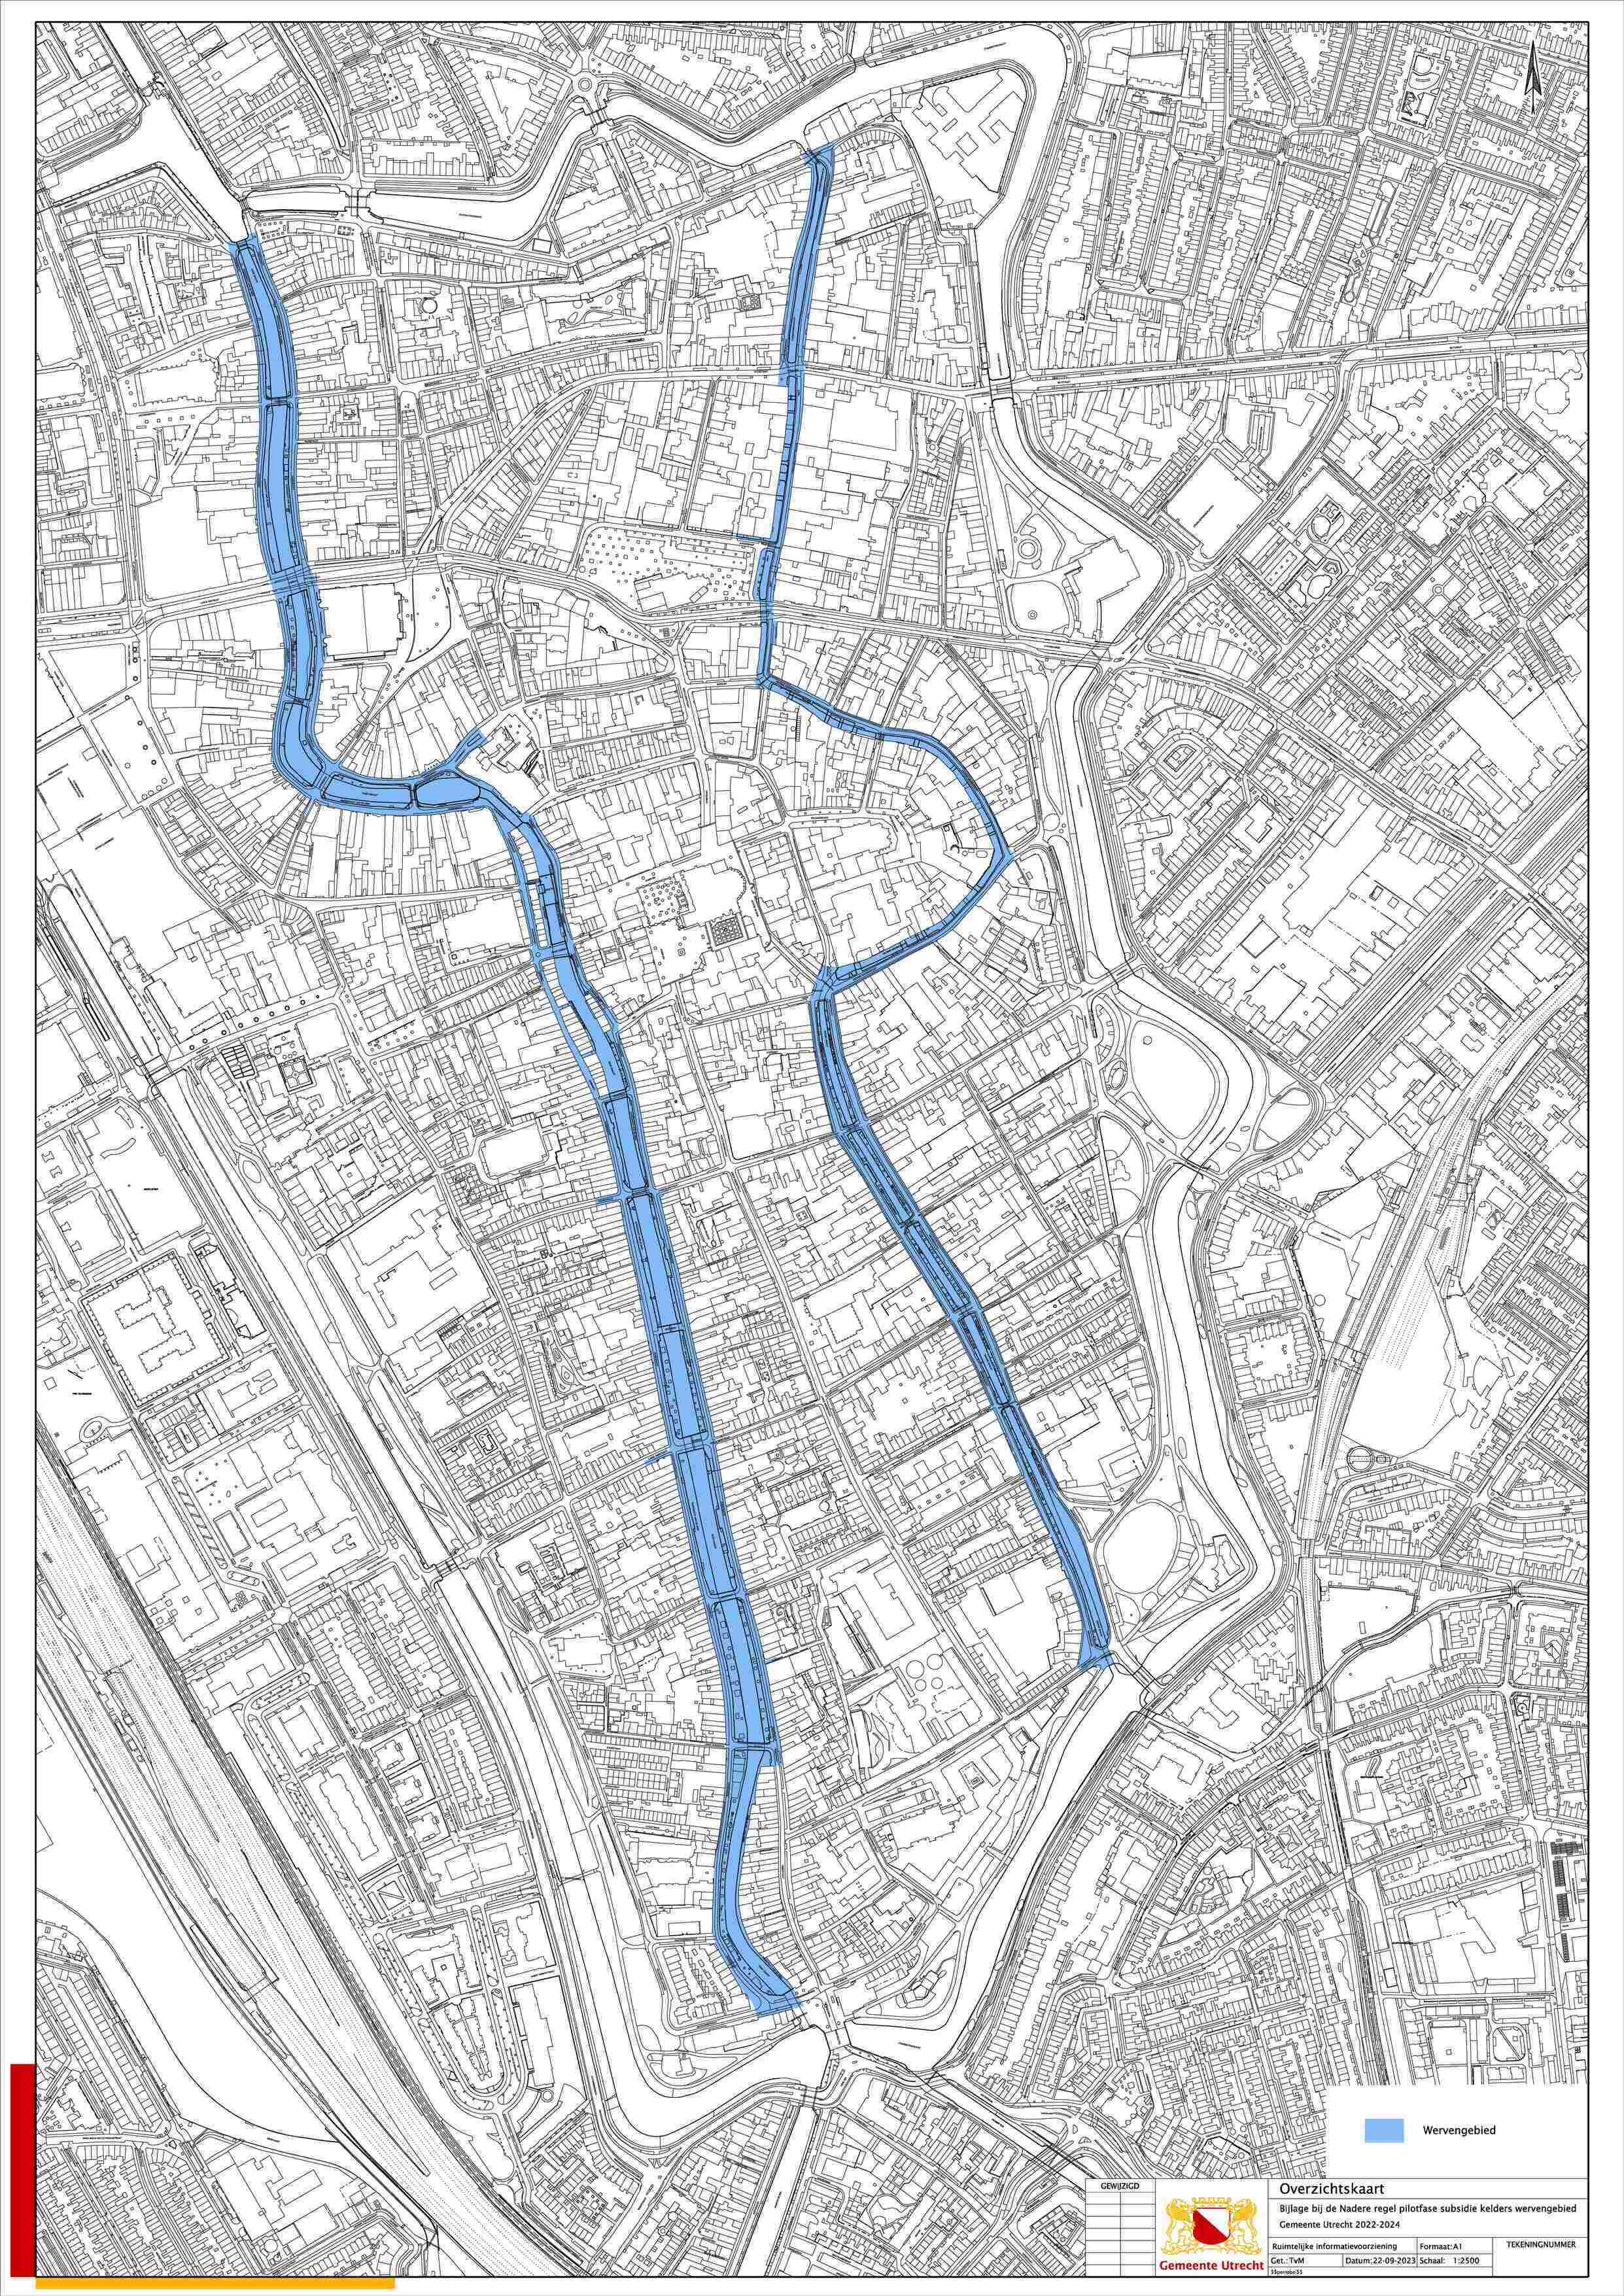
\includegraphics[height=5.0cm]{figures/scope_wervengebiedi83195432-e12f-4974-98be-aaff3c72b58c.jpg}\hspace{2mm}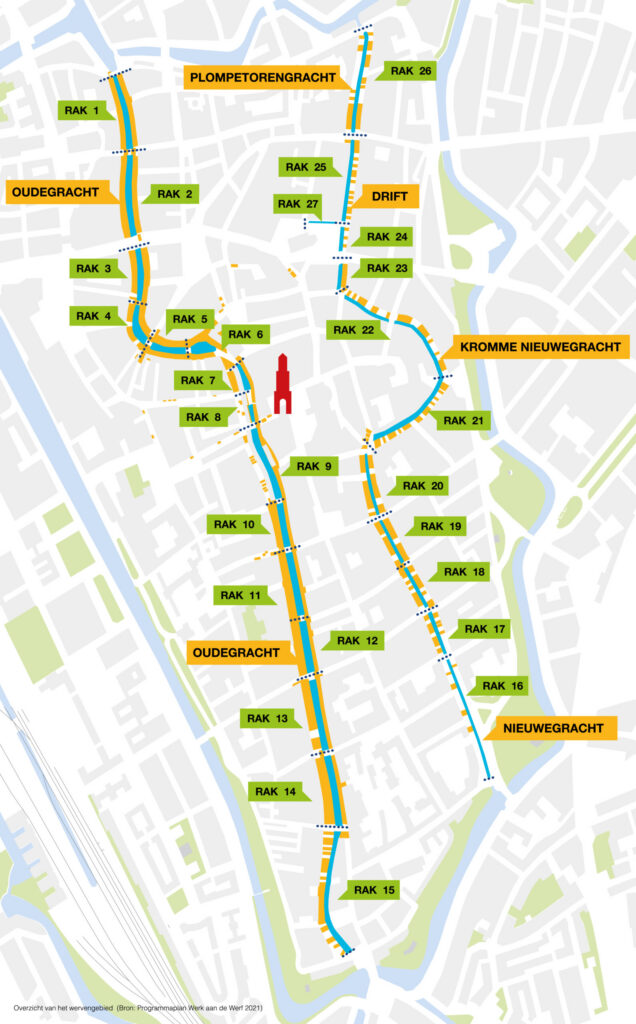
\includegraphics[height=5.0cm]{figures/Plattegrond-wervengebied@2x-scaled-1-636x1024.jpg}
    \captionof{figure}{The Wervengebied: boundary (left) and reaches (\textit{raks}) 1--27 (right). Sources: Gemeente Utrecht (2023); Werk aan de Werf (2021).}
    \label{fig:wervengebied}
    \vspace{-8pt}
\end{wrapfigure}

The Municipality of Utrecht asked our team for a method that supports long-term maintenance decisions for its quay walls. Utrecht has more than 60 km of quay walls and sheet pile walls \parencite{utrecht_teamchallenge2026}. Maintenance is mostly planned on a theoretical end of life, which can differ from the real condition. Money and specialists are limited and the city must stay accessible. Acting too early wastes money. Acting too late is unsafe.

Our goal is a method that sorts quay wall sections by risk and advises a measure (monitoring, restricting use, strengthening or replacement) and an order. It follows the approach of Amsterdam (ARK) and shows where data are missing.

We test the method in the Wervengebied. This is the medieval wharf area along the Oudegracht, Nieuwegracht and Kromme Nieuwegracht (Figure~\ref{fig:wervengebied}). We look at the walls between the water and the wharf. They are about 3.8 km long and divided into 27 reaches (\textit{raks}). Wharf cellars and bridges are left out.

Many of these walls are masonry on timber piles. The city restores about 100~m of wall a year until 2050 \parencite{utrecht_herstelwerven}. Budget and capacity set this pace, not the condition of the walls. The order of work is therefore a real choice.

Inspection can reduce the uncertainty about the wall and the bed level. Traffic, trees, rain and mooring cannot be influenced. Cables, heritage permits and the budget limit the options.

\definecolor{catgreen}{HTML}{4CAF50}
\definecolor{catorange}{HTML}{F59E0B}
\definecolor{catred}{HTML}{DC2626}

\begin{tikzpicture}[
    node distance=12mm and 10mm,
    font=\small\sffamily,
    decision/.style={diamond, aspect=2.2, draw, thick, fill=gray!8,
                     align=center, inner sep=1pt, text width=28mm},
    process/.style={rectangle, rounded corners=2pt, draw, thick, fill=gray!8,
                    align=center, minimum height=9mm, text width=32mm},
    start/.style={rectangle, rounded corners=6pt, draw, thick, fill=gray!20,
                  align=center, minimum height=8mm, text width=30mm},
    category/.style={rectangle, rounded corners=4pt, draw=#1!70!black, thick,
                     fill=#1, text=white, font=\small\sffamily\bfseries,
                     align=center, minimum height=9mm, text width=24mm},
    arrow/.style={-{Stealth[length=2.5mm]}, thick},
    lbl/.style={font=\footnotesize\sffamily, fill=white, inner sep=1.5pt}
]

% Nodes
\node[start] (start) {Quay wall\\ (section)};
\node[decision, below=8mm of start] (life) {Past design\\ life?};
\node[category=catgreen, right=18mm of life] (green) {GREEN};
\node[decision, below=14mm of life] (mas) {Masonry\\ wall?};
\node[category=catorange, right=18mm of mas] (orange1) {ORANGE};
\node[process, below=12mm of mas] (pf) {Calculate failure\\ probability $P_f$};
\node[decision, below=12mm of pf] (thr) {$P_f > P_{f,\mathrm{target}}$?};
\node[category=catred, below left=14mm and 2mm of thr] (red) {RED};
\node[category=catorange, below right=14mm and 2mm of thr] (orange2) {ORANGE};

% Edges
\draw[arrow] (start) -- (life);
\draw[arrow] (life) -- node[lbl] {No} (green);
\draw[arrow] (life) -- node[lbl] {Yes} (mas);
\draw[arrow] (mas) -- node[lbl] {No} (orange1);
\draw[arrow] (mas) -- node[lbl] {Yes} (pf);
\draw[arrow] (pf) -- (thr);
\draw[arrow] (thr.west) -| node[lbl, pos=0.25] {Yes} (red.north);
\draw[arrow] (thr.east) -| node[lbl, pos=0.25] {No} (orange2.north);

\end{tikzpicture}

\newpage
\section{Assumptions, Data Collection and Generation}
\label{sec:assumptions}






The analysis gives a probability of failure $P_f$ and a reliability index
$\beta$ for each walmuur (the low wall between the werf and the canal) that
still stands on its original timber pile foundation. This needs, per wall:
whether the foundation has been renewed, the geometry of wall and foundation,
the retained height, the soil and water behind the wall, the load on the werf
and the condition of the timber piles. The municipal asset register lists the
walls, their length and age, but none of the structural data. We therefore
collected open data and project documents, derived the missing values with
scripts, and filled the remaining gaps with stated assumptions. Within the
time of the project, no data were requested from the municipality.

\subsection{Data collected}\label{sec:data-collected}

Table~\ref{tab:data-sources} lists the data, what each source provides and its
main weakness.

\begin{table}[htbp]
\centering
\small
\caption{Data used for the walmuren, with source and main limitation.}
\label{tab:data-sources}
\begin{tabularx}{\textwidth}{@{}>{\raggedright\arraybackslash}p{2.5cm}
  >{\raggedright\arraybackslash}p{4.3cm}
  >{\raggedright\arraybackslash}X >{\raggedright\arraybackslash}X@{}}
\toprule
Data need & Source & Used for & Limitation \\
\midrule
Walls, length, age & Asset register \cite{gu2025register} & 51 walmuren; screening & No height or foundation data \\
Werf level & AHN 0.5\,m \cite{ahn} & Retained height $H$ & Canal bed not measured \\
Soil & 71 DINO borings \cite{dino} & Soil class, sets $K$ and $\gamma$ & 20--144\,m away; often disagree \\
Groundwater & BRO wells \cite{bro_gmw} & GHG and GLG & Nearest well 143--418\,m \\
Traffic & BGT, NDW \cite{bgt,ndw} & Road distance, axle limit & Road is not on the werf \\
Foundation & Programme reports \cite{antea2019,gu2025up} & Renewed or timber & 8 walls unclear \\
Wall type & TNO dive notes \cite{tno2009} & $P(\text{type 2})$ per rak & Not known per wall \\
Section, piles & \cite{erfgoed156,erfgoed158,ibu2010} & Shapes, levels, piles & Schematic; Oudegracht \\
Timber, method & Hemel \cite{hemel2023,hemel2024} & Pile strength, decay, load & Amsterdam piles \\
Target $\beta$ & NEN 8700 \cite{nen8700} & 1.8 / 2.5 / 3.3 & Class not chosen \\
\bottomrule
\end{tabularx}
\end{table}

The foundation data decide which walls are modelled at all. Of the 51
walmuren, 32 are already renewed on steel, including 11 of the 29 that the
register marks as past their design life. Of the 19 on timber, 2 have no werf:
the street runs to the water, which is a different structure. This leaves 17
walls (611\,m) for the $P_f$ calculation (Appendix~\ref{app:data}).

\subsection{Data generation}\label{sec:data-generated}

Eight scripts turn the raw data into one input row per wall. They run in a
fixed order, each reading the output of the one before
(Appendix~\ref{app:data}). The main generated values are:
\begin{itemize}\setlength{\itemsep}{0pt}\setlength{\parskip}{0pt}
  \item \textbf{Werf level and $H$:} the median of six AHN points on the werf
    side of the wall (+0.99 to +1.57\,m NAP). $H$ is the werf level minus the
    wall underside at $-0.08$\,m NAP \cite{erfgoed158}; median 1.22\,m.
  \item \textbf{Soil class:} the share of clay-like and sand-like soil between
    werf and wall underside in the nearest boring within 250\,m. At least
    70\,\% of one kind gives that class, otherwise ``mixed''. Of the 51 walls,
    23 are clay/peat, 16 sand and 12 mixed.
  \item \textbf{Foundation status:} a hand-compiled table of renewals per rak
    and bank, linked to the register through the city's \emph{Werfmuren} map.
  \item \textbf{Wall type:} divers found a timber beam (\emph{watersloof}, only
    in type 1) or a concrete floor (only in type 2) in some rakken
    \cite{tno2009}, which gives a chance of type 2 per rak.
  \item \textbf{Monte Carlo samples:} 400{,}000 draws per wall and wall type,
    with a fixed seed, for 2026 and 2041 (end of the 15-year reference period
    of NEN 8700).
\end{itemize}
Every raw file is listed with its source and download date, so all results
can be regenerated from the raw data.

\subsection{Assumptions}\label{sec:data-assumptions}
Where no data exist we use the assumptions in Table~\ref{tab:assumptions}.
Uncertain values get a distribution, not a single value. All 27 inputs are
listed in Appendix~\ref{app:data}.

\begin{table}[htbp]
\centering
\small
\caption{Main assumptions where data are missing.}
\label{tab:assumptions}
\begin{tabularx}{\textwidth}{@{}l X l@{}}
\toprule
Quantity & Assumption & Basis \\
\midrule
Canal bed & At the wall underside ($-0.08$\,m NAP), so $H$ is a lower bound & \cite{erfgoed158} \\
Wall type & $P(\text{type 2})$: 0.2 (rak 3--6), 0.5 (rak 21), 0.9 (rak 22), 0.8 (rest) & \cite{tno2009,erfgoed156} \\
Cross-section & Two measured drawings for all walls; floor level $\pm0.15$\,m & \cite{erfgoed156,ibu2010} \\
Pile condition & Soft shell $U(0,45)$\,mm, all walls; grows 0.10--0.25\,mm/yr & \cite{hemel2023} \\
Piles & Diameter $N(180\,\text{mm}, 0.10)$; spacing $U(0.8, 1.2)$\,m & \cite{ibu2010,hemel2023} \\
Soil & $K$ lognormal and $\gamma$ normal per class, independent & Group report, Tab.~C.5 \\
Water & Canal +0.6\,m NAP; groundwater $U(+0.5, +0.9)$\,m NAP & \cite{erfgoed158} \\
Surcharge & $q \sim N(7\,\text{kPa}, 0.20)$ at a distance $U(0,3)$\,m & \cite{hemel2024} \\
Proven strength & Keep only the draws in which the wall stands today & \cite{hemel2024} \\
\bottomrule
\end{tabularx}
\end{table}

\subsection{Effect on the results and validation}\label{sec:data-effect}

The assumptions do not affect the results equally. In order of effect on
$\beta$ (interpreted further in Section~4.2):
\begin{enumerate}\setlength{\itemsep}{0pt}\setlength{\parskip}{0pt}
  \item \textbf{Wall type.} For the same wall, type 1 gives a $\beta$ that is
    1.4--2.4 lower than type 2. With the chance per rak, $\beta$ is 0.1--1.5,
    so all 17 walls are below 1.8. If all were type 2, 7 of the 17 would pass
    1.8. Whether a wall passes therefore depends mostly on its type, which the
    original drawings or a dive inspection can settle.
  \item \textbf{Pile condition.} For type 2 the piles fail far more often than
    the wall overturns (median $P_f$ 0.075 against 0.004). The same broad
    shell is used for every wall, so it shifts all $P_f$ but not the ranking.
  \item \textbf{Retained height and soil.} The soil moment grows with $H^3$:
    0.1\,m more height adds about 25\,\%. As $H$ is a lower bound, this
    assumption makes $P_f$ too low. Clay/peat gives 43\,\% more soil load than
    sand, and nearby borings agree for only 9 of the 51 walls.
  \item \textbf{Surcharge.} 7\,kPa is heavy for a pedestrian werf, so this
    assumption makes $P_f$ too high.
\end{enumerate}

We checked the data and assumptions where possible. The median AHN werf level
on the Oudegracht (+1.13\,m NAP) matches the +0.95 to +1.15\,m NAP measured in
\cite{erfgoed156,erfgoed158}. The renewed length in our foundation table
(about 3.36\,km) matches the city's 3{,}356\,m. The strongest check is that all
17 walls stand today. A first model that treated the wall as a masonry block
gave $P_f \approx 1$ and was rejected. With the measured sections, a type-2
wall stands in 87--100\,\% of the draws, a type-1 wall in only 10--98\,\%.
Either the type-1 model is conservative or many of these walls are type 2; the
proven-strength update accounts for this.

Settlement from pile rot, the damage actually seen on these walls
\cite{erfgoed156}, and failure of the timber screen are not modelled. The
$\beta$ values should therefore be read as an indicative ranking and order of
magnitude, not as exact values. The data that would improve them most are the
wall type per wall, the measured pile condition and canal soundings.


%% ----------------------------------------------------------------------
%%  MAX 2 PAGES  |  RUBRIC WEIGHT 10%
%%
%%  TASK DESCRIPTION
%%  Describe and represent the needed data and how it is relevant to the
%%  problem identified in Section \ref{sec:problem-synthesis}. You may
%%  consider references in data records, literature, or stakeholder
%%  elicitation.
%%  Generate other data that you need. Explain the process and the input
%%  data to guarantee reproducibility of your results.
%%  Indicate sound assumptions to support the problem analysis when data
%%  is not available.
%%  Link to the interpretation of the results in Section
%%  \ref{sec:results-recommendations} and reflect on to what extent the
%%  lack of data accuracy or the uncertainty associated with the data
%%  assumptions may impact your analysis and results. Discuss and validate
%%  the use of the assumptions in the analysis.
%%  This section provides an overview. Use the appendices for supporting
%%  information.
%%
%%  CHECKLIST (challenge task 2: assemble the evidence and confront theory
%%  with observed performance)
%%   - Build a small structured dataset of the assets in your scope from
%%     public sources, and document its provenance, completeness and known
%%     errors. A data quality table is often more informative than the
%%     data itself.
%%   - Exploit proxy data: satellite-based deformation from the
%%     bodemdalingskaart, groundwater levels from the BRO, tree registers,
%%     traffic counts, dredging and water-level records, street-level
%%     imagery over time.
%%   - Take one asset and contrast its code-based assessment outcome with
%%     its observed service history; state what the discrepancy implies
%%     for the rest of the portfolio.
%%   - Consider inspection and monitoring records, field and proof
%%     testing, documented failures elsewhere, and the 'proven strength'
%%     implied by decades of survival under load.
%%   - Reflect on how the gaps in this evidence limit what you can
%%     conclude.
%%
%%  NOTE: the team may submit ONE concrete and justified data request to
%%  the Municipality of Utrecht through the teaching team. Provision is
%%  not guaranteed, so the analysis must also work without it.
%% ----------------------------------------------------------------------


\section{Problem Exploration and Dimension Reduction}

\label{sec:dimension-reduction}

%% ----------------------------------------------------------------------
%%  MAX 1.5 PAGES  |  RUBRIC WEIGHT 5%
%%
%%  TASK DESCRIPTION
%%  Identify the variables playing a role in your problem and analyse how
%%  their levels of variability and uncertainty might affect the final
%%  result.
%%  Reflect on the results. For example: to what extent does a specific
%%  variable really change the results? Do the results correspond to your   
%%  beliefs? How does the lack of accuracy of the data you use affect the
%%  results? Which datasets require more attention, and which estimations
%%  can be made without a significant loss of credibility in the
%%  conclusion?
%%  Decide which variables deserve more effort to reduce their variability
%%  and indicate those whose variability can be neglected.
%%  Justify the process and the use of specific tools for the analysis.
%%
%%  CHECKLIST (challenge task 3: establish which variables drive the
%%  outcome)
%%   - Run a sensitivity analysis and be clear about what your chosen
%%     method can tell you.
%%   - Reduce the problem deliberately: fix variables at defensible
%%     values, aggregate assets into homogeneous classes, or represent a
%%     stretch by a few characteristic cross-sections. Justify each
%%     reduction and estimate what accuracy it costs.
%%   - Turn the result into an inspection strategy: which measurement
%%     would most reduce the variance of your output, and on which assets?
%%     This is the municipality's own question, given more than 60 km of
%%     structures and a limited inspection budget.
%% ----------------------------------------------------------------------


We screen inputs on three outputs: Pf, P(red) and the rank of the 27 reaches Pf is continuous and suited to variance-based indices; the class and rank are discrete, so there we test how many reaches change class when an assumption (A2,A4,A6) is varied. Variables with a total-order index below x are fixed at a defensible value; the remaining n variables are carried as random variables in chapter 2.


Screening variables (determine green/orange): 

- year of construction or last restoration, hence age - asset inventory, available

- design life (100 year, A2) - assumption

- wall type / material (masonry or not) - asset inventory

- foundation type (timber piles, A4) - assumption


Variables for the failure probability Pf (only masonry beyond design life):

- pile diameter - literature value

- decay rate - literature value

- timber strength - literature value

- load (traffic/surface) - literature and traffic data

- groundwater level - nearest BRO well

-soil and surface characteristics - PDOK, BRO


tornado method 


The performance of quay walls and other retaining structures are largely influenced by a number of structural, environmental and demand. This section breaks down the key variables determining the life of quay walls in Utrecht and thus governing the programming of their maintenance. It outlines the influence of the variables on the decisions about the inspection and scheduling of the required intervention, based on their levels of uncertainty in data availability and reasonable assumptions as described in section 1.2.
The aim is to reduce complex asset management programming into a set of measurable variables whose weights and probabilistic projections inform risk of failure by extension aid in scheduling of intervention works. The outlined variables therefore form the basis for the probability calculations and subsequent risk analysis to quantify the likelihood and consequences of potential failure and used to prioritise appropriate maintenance interventions.
The variables were selected based on their theoretical relevance to the structural performance of quay walls, evidence from previous studies and expected influence on failure. The selection was also constrained by the availability of existing data as well as the monetary and time requirements associated with obtaining additional information through testing.

\subsubsection{Design loads}

For comprehensive asset management, it is imperative to identify the loads the structure was designed to bear so as to provide a reference for determining the capacity and subsequently safety in use and assess potential failure. In the analysis of Utrecht quay walls, the design loads are a key demand variable against which current and projected loads up to 2050 are compared.
The design load establishes the range of demand that the structure was intended to accommodate within its theoretical design life. A key uncertainty is the factor of safety incorporated in the original design and its relationship with the safety requirements related to actual loading. Rather than assuming that the historical factor of safety remains directly applicable, sensitivity analysis can examine how reducing or varying the original safety margin affects the assessed structural capacity. The historical design demand can therefore be compared with the corresponding resistance under different safety factors. The factors of safety used in the original design, where available or reasonably estimated, are used to determine the relationship between the specified design demand and the theoretical load-bearing capacity. The resulting range between the original design load and the theoretical maximum at the end of life provides the basis for assessing how changes in demand may influence the probability and timing of failure.


\subsubsection{Traffic Loading}

The loads applied to quay walls over their service life include permanent loads from the self-weight of the structure and earth pressure from retained soil, together with variable loads such as wind, water-current and traffic loads. Traffic loading is associated with relatively high uncertainty because it varies with traffic volume, vehicle composition and changes in demand over time. For uniform analysis, traffic demand is characterised using annual average daily traffic (AADT), while national vehicle-weight data are used to estimate peak traffic loading.
Traffic loading is not treated as the total loading condition of the quay wall and is therefore not directly assessed against the total design load as an isolated variable. Instead, its uncertainty and relationship with the overall structural capacity are modelled to determine its contribution to the probability of failure. Sensitivity analysis assesses how changes in traffic loading influence this probability. Future traffic demand is projected to 2050 and beyond using both annual and local traffic-growth rates, allowing the relationship between increasing traffic demand and available structural capacity to be examined over time. This provides a basis for assessing whether traffic access restrictions could reduce the probability of structural failure in future.


\subsubsection{Soil Type}

The type of soil influences quay-wall behaviour through its geotechnical properties that can influence deformation and structural behaviour such as differential settlement due to variations in ground behaviour. The analysis considers soil type with reference to expansive behaviour that informs consolidation and wetting and drying effects on strength. These are best estimated based on the relation with measurable soil properties of density, cohesion and friction angle.
Expansive soils undergo volume changes with variations in moisture which alter soil properties. Consolidation can result in progressive settlement under sustained loading, potentially contributing to differential movement. These ground responses are to assess how changes in soil behaviour affect the response of the quay wall.
For dimension reduction, sensitivity analysis is used to determine the extent to which uncertainty in soil characteristics and behaviour influences the predicted structural response and failure probability. 


\subsubsection{Structural Material}

Material type is a key variable because the quay-wall portfolio comprises different structural materials, principally timber, steel, concrete and masonry, each with different deterioration mechanisms and rates. Material therefore influences the expected development of structural condition and the remaining capacity of the asset over its service life.

The deterioration rate of each material is considered in relation to the environmental conditions to which it is exposed. In particular, wetting and drying and groundwater conditions may influence the rate and nature of material deterioration. The deterioration process is treated as an uncertain variable because the actual condition and rate of deterioration are not readily measurable across the entire portfolio and may vary between structures and exposure conditions.
For dimension reduction, material type is used to establish the expected deterioration behaviour, while the uncertainty in deterioration rate and current condition is incorporated into the assessment. Sensitivity analysis can determine whether differences in deterioration assumptions materially affect the predicted structural performance and failure probability, thereby identifying where further inspection or material-condition data would have the greatest value for maintenance programming.


\subsubsection{Type of Foundation}

The type of foundation is a significant variable in the assessment because it determines the mechanism through which structural loads are transferred to the ground and therefore influences stability. Shallow foundations are more dependent on near-surface soil and groundwater characteristics, while deep foundations can provide greater stability where shallow conditions are unsuitable, although their condition and behaviour are harder to verify.
In the probabilistic model, uncertain properties of condition and settlement response are represented through probability distributions and their dependence on soil and groundwater conditions. Sensitivity analysis can then establish whether foundation-related uncertainty materially affects predicted stability and failure probability and consequently maintenance decisions. Where sensitivity is high, geotechnical investigation should be prioritised else the variable can be simplified without reducing the credibility of the model.


\subsubsection{Previous Maintenance Records}

Previous maintenance records are an important variable because they provide evidence of how a structure has performed, deteriorated and been repaired over time. Historical records can therefore contribute to estimating remaining service life, deterioration rates and the probability that maintenance will be required within a given planning period. In a probabilistic programming model, this information is used to update the probability of failure rather than just using age of the structure to determine remaining structural life, contributing to the confidence of the intervention timelines and procedures.


\subsubsection{Significance of variables}

Not all variables identified above contribute equaly in the final failure probability. Chapter~\ref{chapter:probabilistic-modelling} shows that pile diameter has the greatest influence in the model, with an influence coefficient $\alpha^2$ of 0.73, against 0.14 for soil and 0.06 for surface load (Appendix~\ref{app:pm-calibration}). Thus, pile geometry is the dominant physical variable, while soil uncertainty remains relevant and surface load has a smaller direct influence. Assumption A1 and foundation type are also important at the portfolio level, although foundation type is not quantified directly in the current timber-pile model.

\textbf{Soil Type} and groundwater conditions are significant mainly through their effect on deterioration rather than through the load directly: Section~\ref{sec:probabilistic-models} shows that a dry groundwater regime lowers the reliability index $\beta$ from 1.41 (moderate) to 0.93, and to 0.81 under the KNMI'23 climate shift, because fungal decay becomes active in a much larger share of samples. \textbf{Structural Material} is significant at the scope level rather than within the current model: the timber-pile mechanism analysed here does not apply to the steel and concrete sections elsewhere in the portfolio (Assumption~A12), so material type determines which model applies before it can influence any single failure probability.

\textbf{Previous Maintenance Records} are significant less for the base failure probability and more for how much that probability can be revised: Section~\ref{sec:probabilistic-models} shows that survival of a known load raises $\beta$ at the moderate location from 1.41 to 2.22, a larger shift than most of the modelling assumptions produce on their own. Variables with little direct influence on the ranking, are fixed at a defensible value rather than treated as a full random variable, since this does not materially change the result.


%\subsubsection{Sensitivity Analysis}Two complementary tools are used: a tornado analysis first screens the candidate variables to remove those with negligible influence, so that computational effort is spent on the ones that matter. The influence coefficients reported in Appendix C.1 are estimated from the standardised input values in the simulated failure samples.This analysis is applied at two levels. At the level of a single section, it identifies which physical variable a measurement should target first: since pile diameter carries by far the largest share of the variance, Section~\ref{sec:probabilistic-models} concludes that a direct diameter measurement is worth more than a refined soil model. At the level of the assumptions themselves, the same logic is applied to A1, A2 and A5 (Section~\ref{sec:data-quality}): each is varied within its stated range, and the resulting change in $\beta$ and in the section ranking is compared against the change produced by the physical variables. Where an assumption shifts the ranking by as much as, or more than, a genuine physical variable, it is flagged as a priority for the municipality's data request rather than left as a fixed input.The three groundwater scenarios in Figure~\ref{fig:pm-results}a are a direct product of this analysis: they were selected because groundwater level drives both the load path (through $k_w$) and the deterioration path (through fungal decay), so its effect could not be adequately summarised by a single sensitivity coefficient and is instead shown as a full scenario comparison.\subsubsection{Justification of Analysis Tools}



\section{Approach Selection}
\label{sec:approach-selection}


The approach is a coarse-to-fine screening of the quay-wall sections, shown in \hyperlink{figure.caption.5}{Figure~1.2}. It is based on the Amsterdam ARK method~\cite{ark2023}. Cheap rules based on the asset register sort the whole portfolio first. The expensive probabilistic analysis is used only where it can change a decision. This suits the problem in \hyperlink{section.1.1}{Section~1.1}. Utrecht holds basic asset data for every section, such as construction year, restoration year and wall type. It does not hold foundation data, pile dimensions or design calculations for the Wervengebied (\hyperlink{section.1.2}{Section~1.2}). Running a detailed deterministic recalculation of all 27 reaches is therefore not possible with the data we have. A purely qualitative ARK score would also fall short, because it does not quantify uncertainty.

\paragraph{Step 1 -- Rule-based screening.}
The theoretical end of life of each section is the year of construction or last full restoration plus a design life of 100 years (A2). If this falls after 2030, the section is classified green and goes into regular maintenance (A3). We chose 2030 because that is when the municipal inspection programme ends~\cite{utrecht_teamchallenge2026}. Sections that reach their end of life by 2030 are then screened on material. Non-masonry walls are classified orange: their deterioration (corrosion, concrete degradation) needs a different model and further inspection. Masonry walls on timber piles (A4) go on to Step~2. This is the most common typology in the scope, and its capacity is the most variable and the least well documented.

\paragraph{Step 2 -- Probabilistic failure model.}
For masonry walls, the failure probability $P_f$ of lateral foundation failure is calculated over the 15-year reference period of NEN~8700~\cite{nen8700} (\hyperlink{chapter.2}{Chapter~2}). We use crude Monte Carlo simulation ($n = 10^6$) instead of FORM, for four reasons:
\begin{itemize}
    \item the limit state is strongly non-linear in the pile diameter;
    \item fungal decay enters through yearly indicator functions of the groundwater level;
    \item dependence between adjacent sections can be imposed directly with a Gaussian copula;
    \item updating with past performance (proven strength) only requires filtering the surviving samples~\cite{hemel2024}.
\end{itemize}
At the $P_f$ levels we are interested in ($10^{-2}$--$10^{-1}$), the computational cost is small. Influence coefficients are estimated from the Monte Carlo design point. We do not have the original pile-group model, so a response function calibrated to Hemel et al.~\cite{hemel2024} replaces it. Because of this, $P_f$ is used to compare sections and scenarios, not as an absolute value.

\paragraph{Step 3 -- Sensitivity analysis and dimension reduction.}
Before the model is applied to all reaches, we screen the inputs (\hyperlink{section.1.3}{Section~1.3}). For the continuous output $P_f$, influence coefficients and scenario runs show which variables matter. Pile diameter dominates, with $\alpha^2 = 0.73$; groundwater acts through decay. For the discrete outputs (class and rank), we use a tornado-type analysis on the assumptions A2, A4 and A6, and count how many reaches change class. Variables with little influence are fixed. Variables with high influence become priorities for inspection, which also informs our data request.

\paragraph{Step 4 -- Consequences and risk classification.}
Consequence indicators are scored from 1 to 4 on the ARK scales (A7)~\cite{ark2023}: traffic function, trees, adjacent buildings and cellars, and quay use. These scores are combined into a consequence score $C$ with explicit weights. Where municipal priorities are unknown, the weights are treated as value judgements and varied in the sensitivity analysis. The consequence level sets the NEN~8700 consequence class. A section is red when $P_f$ exceeds the limit for its class (A6), and orange otherwise. Within each class, sections are ordered by the relative risk $R = P_f \cdot C$.

\paragraph{Step 5 -- Uncertainty in the ranking.}
The uncertain inputs and weights are propagated through the whole procedure, with the same rules applied to every section in each run. The output is therefore a distribution, not a single list: the probability that a reach is red, $P(\text{red})$, its rank distribution, and the probability that one reach outranks another. Assumptions that apply equally to all walls shift every $P_f$ in the same direction, so the ordering is more robust than the absolute values.

\paragraph{Link to the following chapters.}
The red and orange sections feed into the fault tree (\hyperlink{section.3.1}{Section~3.1}). There, structural failure is one causal path next to human and organisational causes of programme failure. The decision tree (\hyperlink{section.3.2}{Section~3.2}) compares interventions for these sections: monitoring, restricting use, strengthening and replacement. Regression (\hyperlink{section.4.1}{Section~4.1}) extrapolates the backlog and risk exposure towards 2050 for different production rates.

% --- Hieronder jullie bestaande figuurcode voor Figure 1.2 laten staan ---


Red: the condition looks so poor that the probability or consequence of failure is too high. This means intensive monitoring and fast follow-up.

Orange: the condition is still unknown and more investigation is needed.

Green: the structure can carry its current use, so regular maintenance is enough.

The steps are:

\begin{enumerate}
    \item Beheerdersoordeel (the asset manager's judgement): a first classification based on limited data.
    \item ARK (Amsterdamse Risicobeoordeling Kademuren): a qualitative risk assessment for orange walls, based on inspections, archives and diver reports. It is done in Excel, and external experts give second opinions.
    \item Herberekening (recalculation) under TAK: for orange walls, the city first decides whether a recalculation is worth it, because it costs a lot of time, money and capacity.
    \item Verfijnd toetsen (refined assessment) under TAK: a more detailed analysis of specific elements.
    \item Integrated management advice for red walls: technical advice is combined with the impact on the surroundings to choose a measure.
    \item Green walls: these go into regular maintenance planning.
\end{enumerate}




The objective is to categorise Utrecht’s quay walls according to their risk of failure, supporting the prioritisation of inspections and maintenance under limited resources. A coarse-to-fine screening approach is adopted, combining rule-based screening with probabilistic analysis. This is suitable because the available asset records and historical inspections provide useful initial information, but incomplete design loads, foundation records and material properties limit the feasibility of detailed deterministic assessment of every structure.

For the initial screening, the theoretical end-of-life year is considered first. Structures with an end-of-life year after 2030 are classified as green, based on the assumption that they are relatively safe and less critical within the study horizon. Structures reaching their theoretical end of life by 2030 proceed to material screening. Masonry structures proceed to detailed analysis while non-masonry structures, including concrete and steel structures, are classified as orange for further inspection. Concrete generally offers higher compressive strength than unreinforced masonry, whose resistance depends on unit and mortar properties (NEN-EN 1996-1-1:2025), while steel has high tensile strength. However, structural capacity depends on capacity and deterioration can lead to loss of strength thus causing uncertainty in materials properties. Masonry structures require immediate in-depth analysis due to their lower and more variable capacity, combined with deterioration-driven loss of strength, creates the greatest uncertainty in structural performance (Materials and Structures,2022).


A probabilistic multi-criteria prioritisation model is selected to rank quay-wall sections by relative risk and assessment urgency.This approach suits the incomplete, heterogeneous information available and provides a reproducible basis for comparing additional sections. An assumption that you apply in the same way to every wall shifts all failure probabilities in the same direction and largely preserves the ordering. That's why the ordering is a robus approach

The technical variables identified in the preceding sections provide inputs to the probabilistic failure model described in Chapter~3. Their effects are represented through the relationships between loading, deterioration and structural resistance, with uncertain inputs described by probability distributions where appropriate. Input assumptions, sources and dependencies will be documented. Consequence indicators will be defined to represent the potential impacts of failure and normalised to a common scale using explicit, justified reference values.

The normalised consequence indicators will be combined using an explicit weighting scheme to obtain a consequence score \(C\). This score will be combined with the model-based failure probability \(P_f\) to calculate a relative risk score, \(R = P_f \times C\), for prioritising quay-wall sections. Literature and relevant guidance will inform the selection and scaling of consequence indicators. The weights will reflect municipal priorities where these can be established; otherwise, they will be documented as value judgements and varied in sensitivity analysis to assess their influence on the ranking.

Monte Carlo simulation propagates uncertainty in inputs and weights through the ranking procedure while preserving specified dependencies. Each run applies common scoring rules and weights to all compared sections. Outputs include score uncertainty, rank distributions and the probability that one section outranks another, conditional on the adopted assumptions.

Global sensitivity analysis will identify which inputs influence the ranking. The results will guide the identification of less influential variables and indicate where additional inspection or data collection could improve confidence in the prioritisation. Assessment of loading variables will also inform the operational interventions considered in the subsequent trade-off analysis.




\begin{figure}[htp]
    \centering
    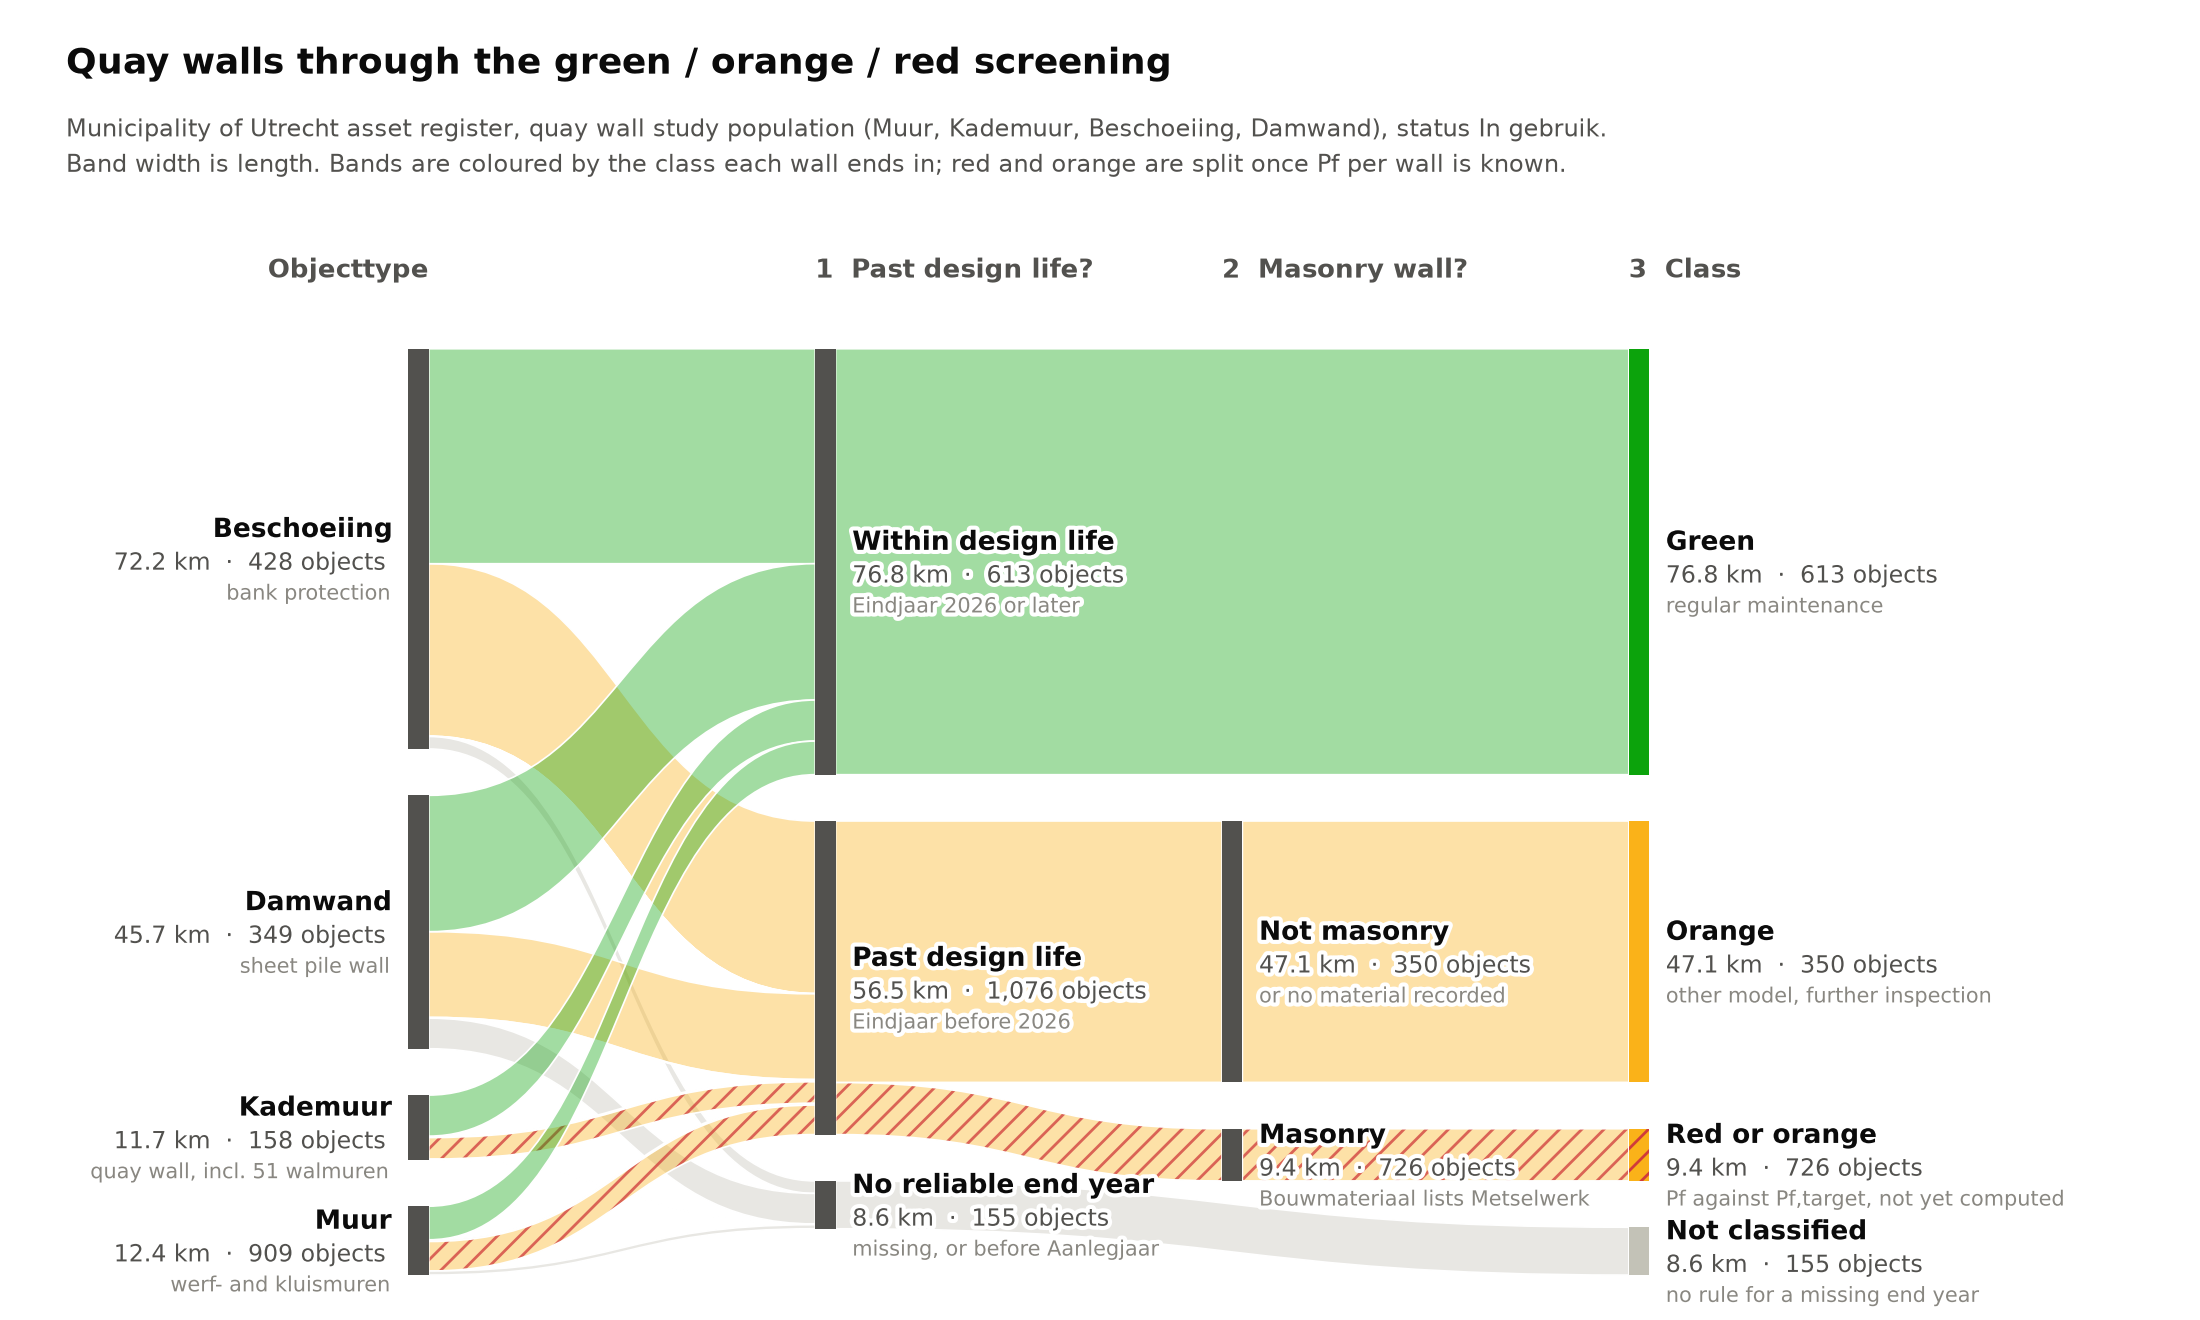
\includegraphics[width=0.75\linewidth]{figures/screening_sankey_register.png}
    \caption{Scoping of the selected area}
    \label{fig:placeholder}
\end{figure}


%% ----------------------------------------------------------------------
%%  MAX 1 PAGE
%%
%%  TASK DESCRIPTION
%%  Explain or represent the approach you will follow to achieve your
%%  goal. You can use a flowchart or graphical representation to convey
%%  the main idea. You can provide both the general picture and a detailed
%%  description of the tools and methods, avoiding definitions of the
%%  methods or other trivial information.

%%  Motivate what modelling tools and uncertainty quantification methods
%%  you choose for the analysis and why. You may compare relevant tools
%%  learned in the course and choose the adequate ones considering the
%%  defined problem and the available data.
%%
%%  NOTE: the challenge tasks are examples, not requirements. If the team
%%  addresses only some of them or takes a different route, that choice
%%  must be justified here.
%% ----------------------------------------------------------------------


\chapter{Probabilistic Modelling}
\section{Probabilistic models}\label{sec:prob}

The risk analysis (Sections~3.1 and~3.2) needs the probability of failure of
each of the 17 walmuren that still stand on timber piles
(Section~\ref{sec:data}). We model it with two limit states, evaluated by
Monte Carlo simulation, and check the model against data and observations.
The full equations are in Appendix~\ref{app:prob}.

\subsection{Limit states}\label{sec:prob-ls}

A wall fails when its body (wall, floor and the soil on it) overturns about
the front pile row, or when a timber pile breaks in bending
\cite{hemel2023,hemel2024}:
\begin{align}
g_1 &= \theta_R M_R + M_\delta - S, \label{eq:g1}\\
g_2 &= \text{MOR} - \left(\theta_M \frac{32 M}{\pi d^3} + \frac{4N}{\pi d^2}\right),
\qquad d = D_0 - 2\bigl(s_0 + r\,(t - 2026)\bigr). \label{eq:g2}
\end{align}
$S$ is the moment of soil, water and surcharge, $M_R$ that of the weight of
the body and $M_\delta$ that of wall friction. $M$ and $N$ act in a pile whose
sound core $d$ shrinks as the rotted shell $s_0$ grows at rate $r$. The wall
fails if either limit state is violated (series system):
$P_f = P(g_1 < 0 \cup g_2 < 0)$ and $\beta = -\Phi^{-1}(P_f)$, estimated as
the fraction of failed draws (400{,}000 per wall and type; 2026 and 2041).

\subsection{Random variables and distributions}\label{sec:prob-variables}

Table~\ref{tab:prob-variables} lists the random variables. Each type of
distribution follows from what is known: a \emph{lognormal} for positive
quantities with a multiplicative error, such as $K$ and the model factors
$\theta$ \cite{jcss2001}; a \emph{normal} for unit weights and timber
properties, where a CoV of at most 0.20 makes negative values negligible; a
\emph{uniform} where only a range is known, as it adds nothing beyond the
bounds; and a \emph{Bernoulli} for the wall type.

\begin{table}[htbp]
\centering
\small
\caption{Random variables of the model. Per wall: values differ between
walls. CoV = coefficient of variation.}
\label{tab:prob-variables}
\begin{tabularx}{\textwidth}{@{}l l l >{\raggedright\arraybackslash}X@{}}
\toprule
Variable & Distribution & Parameters & Estimation \\
\midrule
Werf level (per wall) & Normal & AHN median; $\sigma = 0.05$\,m & AHN data \\
Wall type $T$ (per wall) & Bernoulli & $P(T{=}2)$ = 0.2--0.9 per rak & Dive notes \cite{tno2009} \\
Earth pressure $K$ & Lognormal & 0.35--0.60; CoV 0.20--0.25 & Moments per soil class \\
Soil unit weight $\gamma$ & Normal & 15--18\,kN/m$^3$; CoV 0.05--0.06 & Moments per soil class \\
Surcharge $q$; distance $a$ & Normal; uniform & 7\,kPa, CoV 0.20; 0--3\,m & \cite{hemel2024}; range \\
Groundwater & Uniform & +0.5 to +0.9\,m NAP & Range around canal level \\
Unit weights wall & Normal & 19 / 23\,kN/m$^3$; CoV 0.05 & Typical values \\
Floor level $\Delta z$ & Uniform & $\pm 0.15$\,m & Drawing accuracy \\
Model factors $\theta_R$, $\theta_M$ & Lognormal & mean 1; CoV 0.15, 0.10 & Judgement; JCSS \cite{jcss2001} \\
Pile diameter $D_0$ & Normal & 180\,mm; CoV 0.10 & \cite{ibu2010,hemel2023} \\
Pile spacing $s$ & Uniform & 0.8--1.2\,m & \cite{ibu2010} \\
Soft shell $s_0$; growth $r$ & Uniform & 0--45\,mm; 0.10--0.25\,mm/yr & Measured range \cite{hemel2023} \\
MOR; $E$ & Normal & 22\,MPa, CoV 0.10; 9\,GPa, 0.20 & \cite{hemel2023} \\
Subgrade modulus $k$ & Uniform & 4{,}300--10{,}000\,kN/m$^3$ & \cite{hemel2023} \\
\bottomrule
\end{tabularx}
\end{table}

The parameters are estimated in three ways: from a literature mean and CoV
(method of moments), from our own data (werf level, wall-type prior), and by
Bayesian updating with the observation that every wall still stands (proven
strength \cite{hemel2024}). Draws in which the wall would already fail today
under soil and water alone are rejected; the same evidence updates
$P(T{=}2)$ (Appendix~\ref{app:prob}).

\subsection{Dependence between the variables}\label{sec:prob-dependence}

The dependence is modelled explicitly in four ways:
\begin{enumerate}\setlength{\itemsep}{0pt}\setlength{\parskip}{0pt}
  \item \textbf{Common cause.} The wall type sets the geometry, the floor
    level, the rake of the piles and the head fixity together. The soil class
    sets the means of $K$ and $\gamma$. $P_f$ is a mixture:
    $P_f = \sum_T P(T \mid E)\,P_f(T \mid E)$.
  \item \textbf{Shared variables.} One draw of $K$ enters the soil pressure,
    the surcharge pressure and the wall friction ($\delta = \tfrac23\varphi$,
    with $\varphi$ from $K$). One groundwater level enters the soil weight,
    the water pressure and the buoyancy of the body.
  \item \textbf{Same draws.} Both limit states use the same draws, so their
    correlation is kept: for type 2, overturning and pile failure occur
    together 3.4 times as often as if they were independent. The years 2026
    and 2041 share the piles; only the shell grows.
  \item \textbf{Proven strength.} The check ``stands today'' shares all
    resistance and soil variables with the future load case, but has its own
    groundwater and no surcharge.
\end{enumerate}
Other variables are independent, as no data on their correlation exist. We
tested the two most likely correlations (Appendix~\ref{app:prob}): denser
soil is heavier with a lower $K$, $\rho(K,\gamma) = -0.5$, and stronger timber
is stiffer, $\rho(\text{MOR}, E) = 0.8$ \cite{jcss2001}. Each changes $\beta$
by at most 0.03, mostly upwards, so independence is acceptable and slightly
conservative. The walls are simulated independently, although in reality
they share the uncertain pile condition, surcharge and model factors; this
matters when walls are combined in Section~3.1.

\subsection{Model quality and validity}\label{sec:prob-validity}

Few inputs can be tested against data, but where they can:
\begin{itemize}\setlength{\itemsep}{0pt}\setlength{\parskip}{0pt}
  \item \textbf{Werf level.} AHN points on a werf scatter by about 0.08\,m,
    so the wall average is known to about 0.04\,m, close to $\sigma =
    0.05$\,m. For three walls (Rak 03 OZ, Kromme Nieuwe Gracht 002 and 009)
    the median includes points on stairs or the street, which makes their
    werf 0.3--0.5\,m too high and their $\beta$ too low.
  \item \textbf{Groundwater.} The BRO wells, interpolated to the walls, give
    +0.9 to +2.1\,m NAP, mostly above the werf itself: they stand under the
    raised streets and do not describe the werf, which drains to the canal.
    The range is therefore a physical bound, not a fit. Raising it to
    $U(+0.6, +1.0)$\,m NAP lowers $\beta$ by 0.04--0.09 (type 2) and 0.1--0.4
    (type 1).
  \item \textbf{Soil class.} Only 25--67\,\% of the borings within 150\,m
    give the class of the nearest boring. Treating the class as uncertain,
    with weights from these borings, changes $\beta$ by $-0.7$ to $+0.3$. Walls
    classed as sand lose most, as half of their nearby borings find clay or
    peat. This is the weakest part of the input model.
  \item \textbf{Pile shell.} $U(0, 45)$\,mm has a mean of 22.5\,mm, close to
    the 21\,mm measured in Amsterdam \cite{hemel2023}; no Utrecht data exist.
\end{itemize}

The strongest test is that all 17 walls stand, so a valid model must let
them stand in most draws. A first model that treated the wall as a masonry
block failed in almost every draw and was rejected. With the measured
sections, type 2 stands in 87--100\,\% of the draws and type 1 in only
10--98\,\%: the type-1 model is conservative, or many walls are type 2, and
the update shifts $P(T{=}2)$ accordingly. The Monte Carlo error is small
(CoV of $\hat P_f$ below 2\,\%, $\beta$ within $\pm 0.01$).

The model is valid for low walmuren with a werf on their old timber piles,
for the two Oudegracht cross-sections. It does not cover settlement, sliding
or failure of the timber screen. Because the main inputs are literature
values and ranges, not fits to Utrecht data, the results show the ranking and
order of magnitude of $P_f$ rather than exact values (Section~4.2).

\newpage
%% ----------------------------------------------------------------------
%%  MAX 2 PAGES
%%
%%  TASK DESCRIPTION
%%  To perform the risk analysis in Sections \ref{sec:fault-tree} and
%%  \ref{sec:trade-off}, you need probabilistic models. Identify the
%%  relevant variables and clarify the (in)dependence between them.



%%  Construct adequate probabilistic models with explicit consideration of
%%  the dependence between the variables. You may use uni- or
%%  multivariate probability distributions to describe or quantify the
%%  randomness in the data. You may apply different parameter estimation
%%  techniques.


%%  Justify the selection of the model(s) and evaluate model quality or
%%  validity. For example: does the model fit the data well? To what
%%  extent is the model valid to represent the data?
%%  Use the appendices to add supporting information.
%%




%%  CHECKLIST (challenge task 4: build probabilistic models of
%%  deterioration and demand)


%%   - Represent the relevant degradation processes and their drivers:
%%     groundwater fluctuation and drought acting on timber pile
%%     foundations, bacterial and fungal decay, corrosion, masonry
%%     degradation, scour, and pressure from tree roots.
%%   - Represent the future demands placed on the assets: urban
%%     densification, heavier vehicles and construction traffic, vessel
%%     impact and mooring, and a changing climate (KNMI'23 scenarios
%%     project drier summers, wetter winters and more extreme rainfall).
%%   - Treat dependence between assets and between drivers explicitly
%%     rather than assuming it away.
%%   - Consider that the assessment rules themselves are a source of
%%     uncertainty: they embed safety margins calibrated for new design,
%%     and the margin between calculated and actual capacity is itself an
%%     uncertain quantity worth estimating.
%% ----------------------------------------------------------------------



\chapter{Risk Analysis}
\label{chapter:risk-analysis}

\section{Fault Tree Construction}
\label{sec:fault-tree}

%% ----------------------------------------------------------------------
%%  MAX 3 PAGES
%%
%%  TASK DESCRIPTION
%%  Identify a 'rich' undesired event associated with the failure of the
%%  municipality's quay wall programming to deliver its intended function,
%%  which can be broken down into different causal paths. You may
%%  distinguish the paths from a technical perspective, a human factors
%%  perspective, and/or an organisational perspective. Creativity and
%%  research initiative are appreciated here.
%%  Quantify the occurrence probabilities of the basic events in your
%%  fault tree, based on data records, a literature study, or a structured
%%  expert judgment study.
%%  Propagate the probabilities through your tree, by analytical methods
%%  and/or Monte Carlo simulation in case the basic events might occur due
%%  to (partial) common causes.
%%  Present and interpret the results. For example: do the numerical
%%  results correspond to your beliefs? What are the most sensitive
%%  components in your system? What other data would be needed to
%%  elaborate the trees in further detail?
%%  Discuss the main difficulties encountered with decomposing the system
%%  and processing the data. Explain to what extent data availability or
%%  quality issues may have impacted your analysis. Reflect in particular
%%  on the role of technical, human and organisational factors in your
%%  model, and state under what conditions conclusions can be drawn from
%%  the decomposed system and the collected data.
%%
%%  CHECKLIST (challenge task 5: decompose a 'rich' undesired event)
%%   - Consider candidate top events beyond structural collapse: an
%%     unplanned emergency closure of a quay or street; damage during
%%     works; an asset replaced with decades of life still in it; a
%%     programme so far behind that risk accumulates faster than it is
%%     retired; heritage value destroyed by the very intervention meant to
%%     save it.
%%   - Include human and organisational basic events: an inspection not
%%     carried out or misread; drawings that do not match what is in the
%%     ground; a permit or an owner's consent that never arrives; budget
%%     reallocated mid-programme.
%%   - Quantify basic events from records, literature or elicitation, and
%%     mark clearly the ones for which you had nothing and assumed.
%%   - Handle common-cause failure deliberately: a shared ground profile,
%%     a shared design era, a single inspection contractor, a single
%%     assessment convention applied portfolio-wide.
%% ----------------------------------------------------------------------

The function of the quay wall programme is to keep the walls from failing until
they are renewed. The top event is therefore that the programme does not prevent
the failure of a wall before its renewal, a rich event with technical, human,
organisational and external causes. The team analyses one wall, the median of
the 17 modelled walls, Oude Gracht Rak~09 WZ. Failure means that a limit state of
the model in Section~\ref{sec:prob-ls} is reached; in practice this calls for an
emergency measure or a closure, not necessarily a collapse. At the recent pace
the walls are renewed around 2031 (Section~\ref{sec:regression}), so the tree
covers each wall until its renewal, 5.2 years on average for the median wall,
rather than the 15-year reference period of NEN~8700 \parencite{nen8700}.

\subsection{Structure of the tree}\label{sec:ft-structure}

Figure~\ref{fig:faulttree} shows the tree as it is computed. The top event is
an OR gate with two branches. The first holds the load events that the failure model does not contain (surcharge beyond its range, impact, scour and works), which the programme cannot prevent. The second is an AND gate: a wall fails
only if it reaches a limit state of the model (event LS) and the weakness is
not repaired before the load that breaks it arrives. LS holds the eight causes that the model of Section~\ref{sec:prob} contains: soil (G1), canal bed (G2), groundwater (GW), pile decay (P1, P3), wall type (WT) and masonry (M1, M2). The model combines them through its two limit states, pile bending and overturning; drawn as separate events, they would be counted twice. The weakness is a
present state rather than a slow precursor: the wall type and the soft shell
already decide whether the wall can carry its load, as $\beta$ falls by at most
0.12 in 15 years (Section~\ref{sec:prob-validity}). It can be found in two
ways: by the targeted route, in which the screening sends the wall to a dive with
micro-drilling, or by a regular inspection if the wall shows tilt, cracks or
settlement. It stays unrecognised only if both fail: the targeted route misses
it \emph{and} it gives no visible warning (NW). The repair chain also fails if a
recognised weakness is not acted on or the repair comes too late.

\begin{figure}[ht]
  \centering
  % Generated by scripts/fault_tree_figure.py.
\definecolor{ftT}{HTML}{E3EDFA}\definecolor{ftTb}{HTML}{2A78D6}
\definecolor{ftH}{HTML}{FDEBD9}\definecolor{ftHb}{HTML}{C26A14}
\definecolor{ftO}{HTML}{EFE6F6}\definecolor{ftOb}{HTML}{7C3AED}
\definecolor{ftE}{HTML}{E6F2E0}\definecolor{ftEb}{HTML}{3F7D2A}
\definecolor{ftG}{HTML}{1F2937}\definecolor{ftL}{HTML}{6B7280}
\begin{tikzpicture}[x=1cm,y=1cm,font=\fontsize{6.2}{7}\selectfont,every node/.style={inner sep=1pt}]
\tikzset{gate/.style={draw=ftG,fill=white,rounded corners=1.5pt,font=\fontsize{5}{5}\selectfont\bfseries,minimum width=0.42cm,minimum height=0.22cm},andgate/.style={gate,fill=ftG,text=white},ev/.style={draw=ftG,fill=white,rounded corners=1pt,align=left,text width=1.2cm,minimum height=0.3cm},line/.style={ftL,line width=0.4pt},pv/.style={font=\fontsize{5.6}{6}\selectfont\bfseries,text=ftG}}
\node[draw=ftTb,fill=ftT,rounded corners=1pt,anchor=west,minimum height=0.3cm,text width=4.6cm] at (9.25,0.00) {\textbf{\color{ftTb}W2}\ \ Drainage blocked behind the wall};
\node[pv,anchor=west] at (13.97,0.00) {0.0003};
\node[draw=ftOb,fill=ftO,rounded corners=1pt,anchor=west,minimum height=0.3cm,text width=4.6cm] at (9.25,-0.37) {\textbf{\color{ftOb}Q1}\ \ Traffic heavier than allowed};
\node[pv,anchor=west] at (13.97,-0.37) {0.0017};
\node[draw=ftTb,fill=ftT,rounded corners=1pt,anchor=west,minimum height=0.3cm,text width=4.6cm] at (9.25,-0.74) {\textbf{\color{ftTb}Q2}\ \ Vehicles, terraces or goods at the edge};
\node[pv,anchor=west] at (13.97,-0.74) {0.0003};
\node[draw=ftOb,fill=ftO,rounded corners=1pt,anchor=west,minimum height=0.3cm,text width=4.6cm] at (9.25,-1.11) {\textbf{\color{ftOb}Q3}\ \ Crane or construction traffic};
\node[pv,anchor=west] at (13.97,-1.11) {0.0003};
\node[ev,anchor=west] at (3.70,-0.74) {Surcharge beyond the model};
\node[gate,anchor=west] (g) at (5.06,-0.74) {OR};
\node[pv,anchor=north] at (g.south) {0.0024};
\draw[line] (g.east) -- (5.58,-0.74);
\draw[line] (5.58,-1.11) -- (5.58,-0.37);
\draw[line] (5.58,-0.37) -- (9.25,-0.37);
\draw[line] (5.58,-0.74) -- (9.25,-0.74);
\draw[line] (5.58,-1.11) -- (9.25,-1.11);
\node[draw=ftEb,fill=ftE,rounded corners=1pt,anchor=west,minimum height=0.3cm,text width=4.6cm] at (9.25,-1.48) {\textbf{\color{ftEb}E1}\ \ Vessel impact or mooring overload};
\node[pv,anchor=west] at (13.97,-1.48) {0.0003};
\node[draw=ftTb,fill=ftT,rounded corners=1pt,anchor=west,minimum height=0.3cm,text width=4.6cm] at (9.25,-1.85) {\textbf{\color{ftTb}E2}\ \ Root pressure from trees};
\node[pv,anchor=west] at (13.97,-1.85) {0.0017};
\node[draw=ftTb,fill=ftT,rounded corners=1pt,anchor=west,minimum height=0.3cm,text width=4.6cm] at (9.25,-2.22) {\textbf{\color{ftTb}E3}\ \ Larger scour event};
\node[pv,anchor=west] at (13.97,-2.22) {0.018};
\node[draw=ftEb,fill=ftE,rounded corners=1pt,anchor=west,minimum height=0.3cm,text width=4.6cm] at (9.25,-2.59) {\textbf{\color{ftEb}E4}\ \ Excavation or pipe burst};
\node[pv,anchor=west] at (13.97,-2.59) {0.0003};
\node[ev,anchor=west] at (3.70,-2.04) {Sudden impact, scour or works};
\node[gate,anchor=west] (g) at (5.06,-2.04) {OR};
\node[pv,anchor=north] at (g.south) {0.020};
\draw[line] (g.east) -- (5.58,-2.04);
\draw[line] (5.58,-2.59) -- (5.58,-1.48);
\draw[line] (5.58,-1.48) -- (9.25,-1.48);
\draw[line] (5.58,-1.85) -- (9.25,-1.85);
\draw[line] (5.58,-2.22) -- (9.25,-2.22);
\draw[line] (5.58,-2.59) -- (9.25,-2.59);
\node[ev,anchor=west] at (1.85,-0.92) {Load event beyond the model};
\node[gate,anchor=west] (g) at (3.21,-0.92) {OR};
\node[pv,anchor=north] at (g.south) {0.023};
\draw[line] (g.east) -- (3.73,-0.92);
\draw[line] (3.73,-2.04) -- (3.73,0.00);
\draw[line] (3.73,0.00) -- (9.25,0.00);
\draw[line] (3.73,-0.74) -- (3.70,-0.74);
\draw[line] (3.73,-2.04) -- (3.70,-2.04);
\node[draw=ftTb,fill=ftT,dashed,rounded corners=1pt,anchor=west,align=left,text width=4.6cm] at (9.25,-3.70) {\textbf{\color{ftTb}LS}\ \ Limit state in the model (Section~\ref{sec:prob})\\[1pt]{\fontsize{5.6}{6.6}\selectfont Piles break or wall overturns; contains \textbf{\color{ftTb}G1} soil load, \textbf{\color{ftTb}G2} canal bed, \textbf{\color{ftEb}GW} groundwater, \textbf{\color{ftTb}P1} pile decay, \textbf{\color{ftTb}P3} pile condition, \textbf{\color{ftTb}WT} wall type~1, \textbf{\color{ftTb}M1} masonry, \textbf{\color{ftTb}M2} cross-section}};
\node[pv,anchor=west] at (13.97,-3.70) {0.055};
\node[draw=ftHb,fill=ftH,rounded corners=1pt,anchor=west,minimum height=0.3cm,text width=4.6cm] at (9.25,-4.81) {\textbf{\color{ftHb}S1}\ \ Wrong year or foundation in register};
\node[pv,anchor=west] at (13.97,-4.81) {0.10};
\node[draw=ftOb,fill=ftO,rounded corners=1pt,anchor=west,minimum height=0.3cm,text width=4.6cm] at (9.25,-5.18) {\textbf{\color{ftOb}S2}\ \ Screening rule misses the wall};
\node[pv,anchor=west] at (13.97,-5.18) {0};
\node[draw=ftOb,fill=ftO,rounded corners=1pt,anchor=west,minimum height=0.3cm,text width=4.6cm] at (9.25,-5.55) {\textbf{\color{ftOb}S3}\ \ Model misses the risk};
\node[pv,anchor=west] at (13.97,-5.55) {0.10};
\node[draw=ftOb,fill=ftO,rounded corners=1pt,anchor=west,minimum height=0.3cm,text width=4.6cm] at (9.25,-5.92) {\textbf{\color{ftOb}I1}\ \ Targeted inspection not done in time};
\node[pv,anchor=west] at (13.97,-5.92) {0.30};
\node[draw=ftHb,fill=ftH,rounded corners=1pt,anchor=west,minimum height=0.3cm,text width=4.6cm] at (9.25,-6.29) {\textbf{\color{ftHb}I2}\ \ Damage under water missed};
\node[pv,anchor=west] at (13.97,-6.29) {0.16};
\node[ev,anchor=west] at (7.40,-5.55) {Screening or targeted inspection misses it};
\node[gate,anchor=west] (g) at (8.76,-5.55) {OR};
\node[pv,anchor=north] at (g.south) {0.52};
\draw[line] (g.east) -- (9.28,-5.55);
\draw[line] (9.28,-6.29) -- (9.28,-4.81);
\draw[line] (9.28,-4.81) -- (9.25,-4.81);
\draw[line] (9.28,-5.18) -- (9.25,-5.18);
\draw[line] (9.28,-5.55) -- (9.25,-5.55);
\draw[line] (9.28,-5.92) -- (9.25,-5.92);
\draw[line] (9.28,-6.29) -- (9.25,-6.29);
\node[draw=ftTb,fill=ftT,rounded corners=1pt,anchor=west,minimum height=0.3cm,text width=4.6cm] at (9.25,-6.66) {\textbf{\color{ftTb}NW}\ \ No visible warning before failure};
\node[pv,anchor=west] at (13.97,-6.66) {0.50};
\node[ev,anchor=west] at (5.55,-6.11) {Weakness not recognised};
\node[andgate,anchor=west] (g) at (6.91,-6.11) {AND};
\node[pv,anchor=north] at (g.south) {0.26};
\draw[line] (g.east) -- (7.43,-6.11);
\draw[line] (7.43,-6.66) -- (7.43,-5.55);
\draw[line] (7.43,-5.55) -- (7.40,-5.55);
\draw[line] (7.43,-6.66) -- (9.25,-6.66);
\node[draw=ftHb,fill=ftH,rounded corners=1pt,anchor=west,minimum height=0.3cm,text width=4.6cm] at (9.25,-7.03) {\textbf{\color{ftHb}I3}\ \ Warning not acted on};
\node[pv,anchor=west] at (13.97,-7.03) {0.030};
\node[draw=ftOb,fill=ftO,rounded corners=1pt,anchor=west,minimum height=0.3cm,text width=4.6cm] at (9.25,-7.40) {\textbf{\color{ftOb}L1}\ \ Capacity or budget too small};
\node[pv,anchor=west] at (13.97,-7.40) {0};
\node[draw=ftOb,fill=ftO,rounded corners=1pt,anchor=west,minimum height=0.3cm,text width=4.6cm] at (9.25,-7.77) {\textbf{\color{ftOb}L2}\ \ Heritage permit delays repair};
\node[pv,anchor=west] at (13.97,-7.77) {0.10};
\node[draw=ftOb,fill=ftO,rounded corners=1pt,anchor=west,minimum height=0.3cm,text width=4.6cm] at (9.25,-8.14) {\textbf{\color{ftOb}L3}\ \ Cellar owner consents late};
\node[pv,anchor=west] at (13.97,-8.14) {0.10};
\node[draw=ftEb,fill=ftE,rounded corners=1pt,anchor=west,minimum height=0.3cm,text width=4.6cm] at (9.25,-8.51) {\textbf{\color{ftEb}L4}\ \ Unexpected condition delays repair};
\node[pv,anchor=west] at (13.97,-8.51) {0.10};
\node[ev,anchor=west] at (5.55,-7.96) {Repair comes too late};
\node[gate,anchor=west] (g) at (6.91,-7.96) {OR};
\node[pv,anchor=north] at (g.south) {0.27};
\draw[line] (g.east) -- (7.43,-7.96);
\draw[line] (7.43,-8.51) -- (7.43,-7.40);
\draw[line] (7.43,-7.40) -- (9.25,-7.40);
\draw[line] (7.43,-7.77) -- (9.25,-7.77);
\draw[line] (7.43,-8.14) -- (9.25,-8.14);
\draw[line] (7.43,-8.51) -- (9.25,-8.51);
\node[ev,anchor=west] at (3.70,-7.03) {Weakening not repaired in time};
\node[gate,anchor=west] (g) at (5.06,-7.03) {OR};
\node[pv,anchor=north] at (g.south) {0.48};
\draw[line] (g.east) -- (5.58,-7.03);
\draw[line] (5.58,-7.96) -- (5.58,-6.11);
\draw[line] (5.58,-6.11) -- (5.55,-6.11);
\draw[line] (5.58,-7.03) -- (9.25,-7.03);
\draw[line] (5.58,-7.96) -- (5.55,-7.96);
\node[ev,anchor=west] at (1.85,-5.37) {Limit state reached, not repaired in time};
\node[andgate,anchor=west] (g) at (3.21,-5.37) {AND};
\node[pv,anchor=north] at (g.south) {0.026};
\draw[line] (g.east) -- (3.73,-5.37);
\draw[line] (3.73,-7.03) -- (3.73,-3.70);
\draw[line] (3.73,-3.70) -- (9.25,-3.70);
\draw[line] (3.73,-7.03) -- (3.70,-7.03);
\node[ev,anchor=west] at (0.00,-3.15) {Programme does not prevent a wall failure before renewal};
\node[gate,anchor=west] (g) at (1.36,-3.15) {OR};
\node[pv,anchor=north] at (g.south) {0.048};
\draw[line] (g.east) -- (1.88,-3.15);
\draw[line] (1.88,-5.37) -- (1.88,-0.92);
\draw[line] (1.88,-0.92) -- (1.85,-0.92);
\draw[line] (1.88,-5.37) -- (1.85,-5.37);
\end{tikzpicture}

  \caption{Fault tree for the quay wall programme failing to prevent the failure of a wall before its renewal, as computed for the median wall. OR: at least one input. AND: all inputs together. Numbers: probability of each event and gate, with the load events scaled to the 5.2 years until renewal. The causes inside LS belong to the failure model and are not separate events. Basic events: technical (blue), human (orange), organisational (purple), external (green); bases in Table~\ref{tab:ftprob}.}
  \label{fig:faulttree}
\end{figure}

\subsection{Probabilities of the basic events}\label{sec:ft-probabilities}

Each basic event has a probability for one wall, a range and a basis
(Table~\ref{tab:ftprob}). Of the eight causes inside LS, five are variables of the failure model \parencite{hemel2023,hemel2024}: G1, P1, P3, WT and GW; G2, M1 and M2 enter only through the screen assumption and the model factor $\theta_R$. LS, ``wall reaches a limit state in the model before renewal'', is 0.055 for the median wall (0.15 over 15 years), with a range of 0.033 to 0.46 from the wall being
type~2 or type~1, the largest uncertainty of Section~\ref{sec:dimension-reduction}. The model gives this probability without any
repair and supports only a ranking and an order of magnitude
(Section~\ref{sec:prob-validity}), so using it as a probability is an
assumption. So is spreading the 15-year value evenly over time: the wall type
and the pile condition are a present state, and if the critical load comes
within the exposure, LS approaches 0.15 (Section~\ref{sec:to-results}). The load events are given for 15 years and scaled to the $T_r$ years
until renewal as $1-(1-p)^{T_r/15}$; the human and organisational events are
chances per weakness or per programme and are not scaled. The other events have
one of four bases:
\begin{itemize}
  \item \emph{Data:} S2 is 0, because the screening of
    Section~\ref{sec:approach-selection} flags every wall on its original timber
    piles (Table~\ref{tab:selection}); as the rule was set up on these walls,
    this holds by construction and not for walls elsewhere.
  \item \emph{Derived:} E3 follows from one reported scour case
    \parencite{wijkbericht2024walmuur} among the 51 walls of the register in an
    assumed window of 6 years: $1/(51 \times 6) \times 15 = 0.05$ over 15 years;
    counting only the 19 walls still on timber gives 0.13, near the upper bound.
    L1 follows from the production rate of Section~\ref{sec:regression}: at the
    pace of 2019 to 2026, the 611\,m of the 17 walls are renewed before 2041 in
    more than 99.9\,\% of the bootstrap runs (0.00); only at the lower bound of
    that pace, 22\,m per year, would 45\,\% not be reached.
  \item \emph{Literature:} I2 and I3 are the nominal HEART values for task types C
    (complex, needing skill) and M (miscellaneous)
    \parencite{williams1986heart,heart_table_plos2021}, without error-producing
    conditions; the choice of type is the team's, and plausible conditions would
    raise the top event from 0.049 to 0.052 (Appendix~\ref{app:heart}).
  \item \emph{Assumption:} for the other events no data were found, and the team
    used a fixed scale: extremely rare 0.001, very rare 0.005, rare 0.02,
    occasional 0.10 and likely 0.30. A load event counts only if it occurs
    \emph{and} brings the wall to its limit state; apart from the scour case the
    sources report no such failure, so Q1 and E2 are very rare and the other load
    events extremely rare. NW is 0.5: half of the weak walls are assumed to show
    tilt, cracks or settlement that a regular inspection could see. I1 is 0.30:
    the re-assessment of all quay walls runs until 2030
    \parencite{utrecht_teamchallenge2026}, which covers most of the time until
    renewal, but it need not reach every wall in time; the upper bound, 0.73, is
    the share of the 15-year reference period after 2030 (11 of 15 years).
\end{itemize}

\begin{table}[tbp]
\centering\footnotesize
\caption{Basic events for the median wall. Load events (W2 to E4): probability over 15 years that the event occurs and brings the wall to its limit state, scaled to the years until renewal in the tree. Other events: probability per weakness or per programme.}
\label{tab:ftprob}
\setlength{\tabcolsep}{4pt}
\begin{tabular}{@{}llrll@{}}
\toprule
ID & Event & $p$ & Range & Basis \\
\midrule
LS  & Limit state in the model before renewal & 0.055 & 0.033--0.46 & Model (Sections~\ref{sec:prob}, \ref{sec:regression}) \\
W2 & Drainage blocked & 0.001 & 0.0002--0.005 & Assumption \\
Q1 & Traffic heavier than allowed & 0.005 & 0.001--0.02 & Assumption; occurs \parencite{duic2021} \\
Q2 & Parked vehicles or stored goods & 0.001 & 0.0002--0.005 & Assumption \\
Q3 & Crane or construction traffic & 0.001 & 0.0002--0.005 & Assumption \\
E1 & Vessel hits wall or mooring & 0.001 & 0.0002--0.005 & Assumption \\
E2 & Root pressure & 0.005 & 0.001--0.02 & Assumption; occurs \parencite{duic2020} \\
E3 & Larger scour event & 0.05 & 0.02--0.15 & Derived \parencite{wijkbericht2024walmuur} \\
E4 & Excavation or pipe burst & 0.001 & 0.0002--0.005 & Assumption; occurs \parencite{wijkbericht2025rak5} \\
NW  & No visible warning before failure & 0.50 & 0.30--0.80 & Assumption \\
S1 & Wrong year or foundation in register & 0.10 & 0.05--0.20 & Assumption \\
S2 & Screening rule does not flag wall & 0 & -- & Data (Table~\ref{tab:selection}) \\
S3 & Model misses the risk & 0.10 & 0.05--0.20 & Assumption \\
I1 & Inspection not carried out in time & 0.30 & 0.10--0.73 & Assumption \parencite{utrecht_teamchallenge2026} \\
I2 & Damage under water missed & 0.16 & 0.12--0.28 & HEART type C \parencite{williams1986heart,heart_table_plos2021} \\
I3 & Warning not acted on & 0.03 & 0.008--0.11 & HEART type M \parencite{williams1986heart,heart_table_plos2021} \\
L1 & Capacity or budget too small & 0.00 & 0--0.45 & Derived (Section~\ref{sec:regression}) \\
L2 & Heritage permit delays repair & 0.10 & 0.05--0.20 & Assumption \\
L3 & Cellar owner consents late & 0.10 & 0.05--0.20 & Assumption; occurs \parencite{duic2020} \\
L4 & Unexpected condition delays repair & 0.10 & 0.05--0.20 & Assumption; occurs \parencite{duic2020} \\
\bottomrule
\end{tabular}
\end{table}

Of the 20 events, one comes from the model, one from data, two are derived from
data and two from generic literature; the other 14 are assumptions.
Organisational events such as a delayed permit or a skipped inspection are
recorded only in internal files of the municipality, if at all, and there is no
public register of quay wall incidents; the technical causes with the best
data sit inside LS. The municipality's inspection and incident records,
which it will provide in the case-study phase, or a structured expert judgement would replace
most of them.

\subsection{Propagation and results}\label{sec:ft-results}

For one wall, an OR gate gives $P = 1-\prod_i(1-p_i)$ and an AND gate
$P=\prod_i p_i$ \parencite{vesely1981ftHandbook}. Within one wall, WT and GW sit
inside the model event, where they are drawn once, so their dependence is kept.
For the 17 walls together, each with its own years until renewal and its own LS,
the team used Monte Carlo simulation ($4\times10^5$ runs), because some causes
act on several walls at once. The failure model simulates the walls
independently (Section~\ref{sec:prob-dependence}), so their model events are
linked here with a Gaussian copula and a weak correlation, $\rho=0.084$, a team
judgement for the shared pile age and soil without data.
S3, I1 and I2 are partly shared (the same screening model, programme and
inspectors): 100\,\%, 100\,\% and 50\,\% of their probability is one common draw
for all walls, the rest is drawn per wall. These shares, $\rho$ and the
independence of the load events between walls are assumptions.

For the median wall, the load branch gives 0.023 and ``weakening not repaired in
time'' 0.48. The probability that the programme does not prevent its failure
before renewal is 0.049: 0.015 with all probabilities at their lower bound, 0.47
at their upper bound, where the wall is type~1, and 0.042 to 0.067 over the 17
walls. Without any repair it would be 0.077, so the repair chain lowers it by a
third; if every weakness gave warning (NW~=~0), to 0.039. Over the 17 walls the
expected number of failures before renewal is 0.82
(Figure~\ref{fig:app-fault-tree}). The tree takes the 0.97 model events of
Section~\ref{sec:regression}, lets the repair chain stop half of them, and adds
0.36 from the other load events. Common cause hardly changes the spread
(standard deviation 0.92 to 0.93). Of the 18 minimal cut sets, eight are of order 1
(the load events), five of order 2 (LS with I3 or L1 to L4) and five of order 3
(LS with NW and one of S1 to S3, I1 or I2). The Fussell--Vesely importance
\parencite{fussell1975} is 0.53 for the model event, 0.35 for scour E3, 0.21
for NW, 0.08 for I1 and 0.06 for each of L2 to L4. Moving one probability from
its lower to its upper bound changes the result most for LS (0.20), E3 (0.047)
and L1 (0.013).

\subsection{Interpretation}\label{sec:ft-interpretation}

The results are higher than the incident data suggest. The sources
name about four incidents in the whole Wervengebied between 2017 and 2024: a
temporary support at Oudegracht 110--122 in 2017 \parencite{duic2022}, a partly
closed street on the Kromme Nieuwegracht and a road hole on the Nieuwegracht,
reported in 2020 \parencite{duic2020}, and scour under the wall near the
Bezembrug in 2024 \parencite{wijkbericht2024walmuur}. That is about 0.5 per year
over 4.1\,km of walmuur, or 0.12 per km, all emergency measures, no collapse,
and not all clearly a failure of a walmuur. The tree gives 0.17 per year for the
611\,m of modelled wall, 0.28 per km: more than twice the observed rate.
The incident search was not systematic, so four is a lower bound; the gap fits
a model event on the safe side: the type-1 model is
conservative (Section~\ref{sec:prob-validity}) and 7\,kPa is a heavy load for a
werf (Section~\ref{sec:data-effect}).

The failure model of Section~\ref{sec:prob} gives the technical part of the tree the best support, although its timber properties come from one Amsterdam case; the human part uses generic values and the organisational part mostly
assumptions. A further difficulty was that pile condition is not a yes/no event,
while a missed inspection is; the team used the failure probability of the model
as one event and added NW for the warning it may or may not give. The repair
chain lowers the probability from 0.077 to 0.049, mostly through the targeted
route; the human and organisational events (I1, L2 to L4) matter, but less than
the wall type and scour. Because the range of LS dominates every other swing,
measuring the wall type and the pile condition matters more than speeding up
the repair.

The conclusions hold for the ranking of causes, not for absolute
probabilities. The most useful extra data are the
pile condition from micro-drilling (LS, NW), canal-bed soundings and scour records
(E3), the real programme order (L1 and the years until renewal), and an incident
log of closures and emergency measures to check the result.


% Section 3.2 Trade-off analysis
% Fallback: defines \euro if eurosym is not loaded in the preamble
\providecommand{\euro}{\texteuro}

\section{Trade-off Analysis}
\label{sec:tradeoff}

The team used the fault tree of Section~\ref{sec:fault-tree} to compare
interventions for the median wall until its renewal, 5.2 years at the recent
pace. Each intervention lowers one or more basic events, and the new
probabilities are propagated through the same tree. The decision tree
(Figure~\ref{fig:dtree}) has one decision node with eight alternatives. Seven end
in a chance node with two outcomes: the programme does or does not prevent a
failure, which here means an emergency measure or a closure. The eighth, A7,
first measures the wall and then chooses (a preposterior analysis). The
objective is the lowest expected total cost
\begin{equation}
  E[C_i] = c_i + P_{f,i}\, C_f\, \mathit{DF}_i ,
\end{equation}
where $c_i$ [\euro] is the present value of the cost of intervention $i$, $C_f$
[\euro] the cost of a failure and $\mathit{DF}_i$~\mbox{[--]} the mean discount factor
over the exposure, at 2.8\,\% per year, the standard rate for Dutch social
cost-benefit analyses from 2026 \parencite{discontovoet2025}.

\subsection{Interventions and costs}\label{sec:to-interventions}

Table~\ref{tab:interventions} lists the alternatives: technical, human and
organisational measures, restricting use, renewing now and monitoring.
Strengthening (a relieving floor, new piles or a new screen) is left out: for a
wall renewed within about five years it would cost a large part of a renewal and
then be demolished; for walls that wait much longer it belongs in the tree.
How much a measure lowers an event is not known
from data, so one rule is assumed: a measure moves the events it acts on to the
lower bound of their range in Table~\ref{tab:ftprob}. Two alternatives use the
failure model directly: for A6 it is rerun without surcharge within 1.5\,m of
the edge, which raises $\beta$ of the median wall from 1.05 to 1.31, and for A7
it gives the displacement that a survey would see
(Appendix~\ref{app:prob-checks}). The municipality has high-level unit costs
of replacement \parencite{utrecht_qa2026}; they were not used here, so the
costs below are estimates from published budgets and team judgement in 2026
prices, to be replaced by the municipal figures; cost escalation above
inflation is not modelled and would favour renewing now. Renewing a wall of average length, 36\,m, costs about \euro1.3 million: the programme plan reserves about \euro110 million for the roughly 3\,km of wal- and kluismuren still to be restored, or
\euro35k per metre \parencite{utrecht_programmaplan}. As the wall is renewed
within about five years anyway, renewing now (A4) costs only the present value of bringing that renewal forward, \euro156k, provided extra capacity is
hired; within the same capacity it would delay another wall, which is the order
question of Section~\ref{sec:regression}. The failure cost $C_f = $ \euro1.5
million combines a temporary safety structure of about \euro0.25 million per
wall, from the \euro650k per 100\,m that Amsterdam budgets
\parencite{amsterdam_tender}, \euro0.65 million for the extra cost of an urgent
renewal and \euro0.6 million for closures, damage to cellars and hindrance; as
it is uncertain, it is varied from \euro0.1 to \euro30 million.

\begin{table}[htbp]
\centering
\caption{Decision alternatives for the median wall until its renewal, costed for a wall of average length (36\,m).
T = technical, H = human, O = organisational. New values are lower bounds from
Table~\ref{tab:ftprob}, except those marked *. Costs: one-off plus yearly.}
\label{tab:interventions}
\small
\begin{tabularx}{\textwidth}{@{}llXr@{}}
\toprule
Alternative & Type & Measure and changed basic events & Cost $c_i$ \\
\midrule
A0 Current programme & -- & No extra measures & \euro0k \\
A1 Scour and load control & T & Bed protection and yearly soundings; cameras for the axle limit; root barriers. E3, Q1, E2 & \euro72k + 3k/yr \\
A2 Inspection & H, T & Dive with micro-drilling and a second reviewer; tilt sensors with an alarm. I1, I2, I3, S3; NW 0.50$\to$0.30* & \euro60k + 2k/yr \\
A3 Organisation & O & Share of an extra project leader; agreements with the heritage department and cellar owners; site investigation. L2, L3, L4 & \euro15k + 7k/yr \\
A4 Renew now & T & Renewal in the first year with extra capacity: exposure 5.2$\to$1 year*; E3, W2 & \euro156k* \\
A5 Package & all & A1 + A2 + A3 together & \euro205k \\
A6 Restrict use & O & No terraces, goods or vehicles within 1.5\,m of the edge until renewal. LS 0.055$\to$0.035*; Q1, Q2 & \euro10k + 3k/yr \\
A7 Monitor, then decide & H, T & Survey of the displacement: below 5\,mm keep A0, otherwise A6* & \euro15k (+ A6) \\
\bottomrule
\end{tabularx}
\end{table}

\subsection{Results and preferred alternative}\label{sec:to-results}

Figure~\ref{fig:dtree} gives the results. The
current programme gives $P_f = 0.049$ and an expected cost of \euro68k; $P_f$
has two main parts, the model event that is not repaired in time
($0.055 \times 0.48 = 0.026$) and the load branch (0.023), mostly scour.
Restricting use (A6) lowers $P_f$ by a fifth, to 0.037, at an expected cost of
\euro77k, close to A0. Scour and load control (A1) and inspection (A2) lower it
to 0.035 and 0.041, but cost more than they save. Renewing now (A4) gives the
lowest $P_f$ (0.007). Monitoring (A7) costs \euro83k: the survey finds less
than 5\,mm with probability 0.72, after which $\beta$ rises to 1.54 and the
wall stays in the programme; otherwise $\beta$ falls to 0.36 and use is
restricted.

\begin{figure}[htbp]
\centering
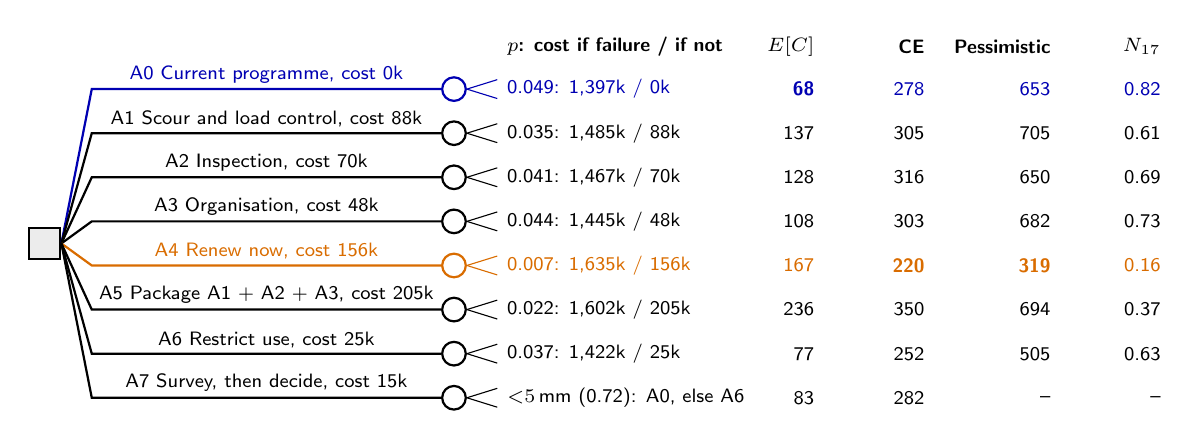
\begin{tikzpicture}[font=\scriptsize\sffamily]
\node[draw, thick, fill=gray!15, minimum size=4mm] (d) at (0,0) {};
\node[right] at (5.75,2.5) {\bfseries $p$: cost if failure / if not};
\foreach \x/\t in {9.9/{$E[C]$}, 11.3/{CE}, 12.9/{Pessimistic}, 14.3/{$N_{17}$}}
  \node[left] at (\x,2.5) {\bfseries \t};
\foreach \idx/\alt/\cst/\pf/\cf/\cn/\ec/\ce/\pe/\n/\col in {
  0/A0 Current programme/0/0.049/1{,}397/0/\textbf{68}/278/653/0.82/blue!70!black,
  1/A1 Scour and load control/88/0.035/1{,}485/88/137/305/705/0.61/black,
  2/A2 Inspection/70/0.041/1{,}467/70/128/316/650/0.69/black,
  3/A3 Organisation/48/0.044/1{,}445/48/108/303/682/0.73/black,
  4/A4 Renew now/156/0.007/1{,}635/156/167/\textbf{220}/\textbf{319}/0.16/orange!85!black,
  5/A5 Package A1 + A2 + A3/205/0.022/1{,}602/205/236/350/694/0.37/black,
  6/A6 Restrict use/25/0.037/1{,}422/25/77/252/505/0.63/black} {
  \pgfmathsetmacro{\y}{1.96-0.56*\idx}
  \node[draw, thick, circle, minimum size=3mm, inner sep=0pt, \col] (c\idx) at (5.2,\y) {};
  \draw[thick, \col] (d.east) -- (0.6,\y) -- node[above=-1.5pt] {\alt, cost \euro\cst k} (c\idx.west);
  \draw[\col] (c\idx.east) -- (5.75,\y+0.12);
  \draw[\col] (c\idx.east) -- (5.75,\y-0.12);
  \node[right, \col] at (5.75,\y) {\pf: \euro\cf k / \euro\cn k};
  \node[left, \col] at (9.9,\y) {\ec};
  \node[left, \col] at (11.3,\y) {\ce};
  \node[left, \col] at (12.9,\y) {\pe};
  \node[left, \col] at (14.3,\y) {\n};
}
\pgfmathsetmacro{\y}{1.96-0.56*7}
\node[draw, thick, circle, minimum size=3mm, inner sep=0pt] (c7) at (5.2,\y) {};
\draw[thick] (d.east) -- (0.6,\y) -- node[above=-1.5pt] {A7 Survey, then decide, cost \euro15k} (c7.west);
\draw (c7.east) -- (5.75,\y+0.12);
\draw (c7.east) -- (5.75,\y-0.12);
\node[right] at (5.75,\y) {${<}5$\,mm (0.72): A0, else A6};
\node[left] at (9.9,\y) {83};
\node[left] at (11.3,\y) {282};
\node[left] at (12.9,\y) {--};
\node[left] at (14.3,\y) {--};
\end{tikzpicture}
\caption{Decision tree for the median wall until its renewal, with the results.
Square: decision node; circle: chance node with the probability $p$ that the
programme does not prevent a failure, from the fault tree of
Section~\ref{sec:fault-tree} with the changed basic events. Costs in \euro k,
present values at 2.8\,\%; $C_f = $ \euro1{,}500k. CE: certainty equivalent with
exponential utility, $R = $ \euro0.5 million. Pessimistic: $E[C]$ with all basic
events at the upper bound of their range in Table~\ref{tab:ftprob} and LS at its
type-1 value ($p$ of A0 0.47); a measure lowers an event by the same factor as
in the base case (assumption). $N_{17}$: expected number of failures among the
17 walls before renewal. Bold: lowest cost per criterion; blue: preferred when
risk-neutral; orange: preferred under both risk-averse criteria.}
\label{fig:dtree}
\end{figure}

A risk-neutral decision maker looks only at $E[C]$, which with $C_f = $ \euro1.5 million favours A0, with A6
\euro9k behind. The choice depends on $C_f$ (Figure~\ref{fig:app-fault-tree}): A6 is the cheapest from
\euro2.4 million, A7 from \euro4.4 million and A4 from \euro5.05 million. A public
owner of heritage walls is more likely risk-averse, which the team tested in two
ways. With an exponential utility function,
$\mathrm{CE} = R \ln E[e^{C/R}]$ with risk tolerance $R = $ \euro0.5 million
(assumption), renewing now has the lowest certainty equivalent (\euro220k
against \euro252k for A6 and \euro278k for A0), because it almost removes the
large loss; with $R = $ \euro1 million A6 is best and with \euro2 million A0.
In a pessimistic scenario with all events at their upper bound and the wall of
type~1, A4 is also the cheapest (\euro319k against \euro505k for A6). The
risk-neutral choice is therefore A0, followed by A6, and the risk-averse choice
A4. These choices depend on the absolute level of $P_f$, which the model does
not give (Section~\ref{sec:prob-validity}). With event LS three times lower, A0
stays the cheapest; with LS three times higher, or without spreading the
15-year value over time (LS = 0.15), A6 becomes the cheapest (\euro124k and
\euro116k against \euro140k and \euro127k for A0). A4 keeps the lowest
certainty equivalent in every case.

The median wall is orange, so Table~\ref{tab:walls-decision} repeats the decision, with the same costs, for a red wall that is probably type~1, Oude Gracht Rak~03
OZ, and for the green wall with the lowest $P_f$, Kromme Nieuwe Gracht 003. For
the red wall, renewed in about 2.6 years, restricting use is already the
cheapest at the base $C_f$ and renewing now is the risk-averse choice; for the
green wall the current programme stays the cheapest up to \euro3.95 million.
This backs the measures per class of Section~\ref{sec:approach-selection}:
restricted use and early renewal for red walls, regular inspection for green
ones.

\begin{table}[htbp]
\centering
\small
\caption{Decision for three walls until their renewal, with the costs of
Table~\ref{tab:interventions}, $C_f = $ \euro1.5 million and $R = $ \euro0.5
million. $T_r$: years until renewal; $C_f^{*}$: failure cost from which
restricting use (A6) is the cheapest.}
\label{tab:walls-decision}
\setlength{\tabcolsep}{4pt}
\begin{tabular}{@{}l l r r c l l r@{}}
\toprule
Wall & Class & $T_r$ [yr] & $P_f$ A0 & $E[C]$ A0 / A6 / A4 [\euro k] & Cheapest & Lowest CE & $C_f^{*}$ [\euro M] \\
\midrule
OG Rak 03 OZ & red & 2.6 & 0.067 & 98 / 95 / 109 & A6 & A4 & 1.3 \\
OG Rak 09 WZ (median) & orange & 5.2 & 0.049 & 68 / 77 / 167 & A0 & A4 & 2.4 \\
KNG 003 & green & 6.7 & 0.044 & 60 / 77 / 209 & A0 & A6 & 3.95 \\
\bottomrule
\end{tabular}
\end{table}

\subsection{Monitoring and the value of information}\label{sec:to-monitoring}

The municipality named monitoring as a source of evidence
\parencite{utrecht_qa2026}. In the model, a type-1 wall has moved 6 to 9\,mm under its soil and water and a type-2 wall 1 to 3\,mm, so a
survey of the horizontal displacement, with an error of 2\,mm, mainly reveals
the wall type, much as a survived load of 10\,kN/m$^2$ with small displacements
raised $\beta$ from 1.5 to 3.2 in \textcite{hemel2024}. For the median wall the survey is worth
nothing before its cost of \euro15k, because the wall is renewed within about
five years and restricting use is a cheap response anyway. For a wall that has
to wait 15 years, as most of the 60\,km will, the same survey is worth \euro3k
at $C_f = $ \euro1.5 million but \euro56k at \euro5 million. Monitoring thus pays
where renewal is far away, which is where the portfolio method uses it
(Section~\ref{sec:approach-selection}). Satellite data measure vertical
movement, which belongs to the settlement mechanism that the model leaves out;
they serve as an indicator, not as an update of $\beta$.

\subsection{Reflection}\label{sec:to-reflection}

The team expected the organisational measures to matter more. They lower $P_f$
by a tenth (A3), because the targeted route already stops half of the failures
of the model and the rest comes from the wall type and scour. The team did not expect restricting use to compete with the
current programme, nor renewing now to win under risk aversion. Both
follow from the short exposure, which favours measures that work at once over
measures whose benefit builds up over years, such as bed protection or an extra
project leader. Not all objectives can be put in euros. $C_f$ has no life-safety
part: on a busy werf, an expected 0.05 fatalities per failure at a value of a
statistical life of about \euro2.2 million in 2001 prices \parencite{deblaeij2003},
some \euro3.5 million today, would add about \euro0.18 million, still below the
\euro2.4 million at which A6 becomes the cheapest. The cost of A6
falls mostly on terrace owners, who lose seats by the water, and the closures
of A4 hinder access to the inner city; these conflicts are not in $C_f$ and need
a political choice.

The inputs differ in quality. Event LS comes from the failure model, whose
inputs are mostly literature values; NW and the organisational events are
assumptions; the effect of A6 is as uncertain as the surcharge itself, and
scour E3 rests on a single case. The costs are team estimates: for the median
wall, a measure would match A0 at \euro15k for restricting use (estimate
\euro25k) but at \euro7k to \euro18k for A1 to A3 (estimates \euro48k to
\euro88k); with all costs of the measures halved A6 becomes the cheapest, and
with a renewal cost 30\,\% higher A6 replaces A4 as the risk-averse choice.
The ranking of the alternatives therefore holds only within the tested range:
A0 and A6 swap places when LS is three times higher or A6 is cheaper, and A4
stays the risk-averse choice unless renewal costs more. The conclusions assume
independent walls, measures that work as soon as they are taken, the
lower-bound rule for their effect, and a renewal within about five years; with
half that effect, A0 stays the cheapest and A6 second (\euro85k).
Because the measures interact through the AND and OR gates, they have to be
judged together, as in A5. The data that would help most are the municipal unit
costs and the costs of emergency measures in Utrecht, to fix $C_f$ and the
costs of the measures; canal
soundings and a scour record, to estimate E3; how often weak walls in Utrecht
showed warning signs, to estimate NW; and the wall type per wall, which would
allow renewing early only the weak type-1 walls.

\subsection{Effectiveness of the interventions}\label{sec:to-effectiveness}

Measured against the current programme, no measure pays for itself in expected
value at $C_f = $ \euro1.5 million for the median wall, whereas restricting use
does for a red wall such as Rak~03 OZ. For the median wall it comes closest: it lowers $P_f$ by a fifth for
\euro25k, under 2\,\% of the cost of a renewal. Renewing now lowers it by 85\,\%
for an extra \euro156k and the package by 55\,\% for \euro205k, whereas
inspection and organisation, at 15 and 10\,\%, are not effective on their own.
For walls renewed within a few years, the effective measures are those that
act at once: restricting use on the red walls, and renewing the weakest first
when extra capacity is available. Monitoring becomes effective for walls that
will wait much longer.

The largest lever is the pace of the programme
(Section~\ref{sec:regression}). Returning to the pace of 2015 to 2018 brings the
renewal of the 17 walls forward, which costs \euro1.2 million in present value
at \euro35k per metre, and avoids 0.42 expected limit states, worth
\euro0.6 million at $C_f = $ \euro1.5 million: it pays only from $C_f \approx$
\euro3 million. At the base failure cost, budget and the accessibility of the city centre, rather than this risk, should set the pace.



%% ----------------------------------------------------------------------
%%  MAX 3 PAGES
%%
%%  TASK DESCRIPTION
%%  The 'rich' undesired event broken down in Section
%%  \ref{sec:fault-tree} is used here to analyse the possible
%%  interventions that reduce its occurrence probability. You may consider
%%  interventions from a technical, human factors and/or organisational
%%  perspective. Creativity and research initiative are appreciated here.
%%  Structure and systematically investigate the interventions in a
%%  decision tree in order to compare the costs and benefits of your
%%  decision alternatives.
%%  Present and interpret the results. For example: do the results
%%  correspond to your beliefs? What are the most effective interventions
%%  in your system? What other data would be needed to elaborate the
%%  decision tree further? Which decision alternative is preferred from a
%%  rational risk-neutral optimisation procedure, and which from a
%%  risk-averse procedure?
%%  Reflect on the procedure and the results. Can all conflicting
%%  objectives be quantified? Discuss the main difficulties encountered
%%  with trading off the objectives and processing the data. Explain to
%%  what extent data availability or quality issues may have impacted your
%%  analysis, reflect on the role of technical, human and organisational
%%  factors, and state under what conditions conclusions can be drawn from
%%  the optimal interventions and the collected data.
%%  To what extent are the proposed intervention measures effective in
%%  reducing the occurrence frequency of undesired events?
%%
%%  CHECKLIST (challenge task 6: compare interventions and programme them
%%  under real constraints)
%%   - Structure the full range of alternatives: doing nothing and
%%     continuing to monitor; restricting use (load limits, traffic
%%     restrictions, closure); maintenance that preserves existing
%%     functionality; life-extension and strengthening (renovation,
%%     foundation improvement, relieving structures, load reduction);
%%     replacement at the end of life; and improvement or expansion that
%%     adds functionality, such as nature-friendly banks, ecological
%%     integration, circular or demountable structures, and climate
%%     adaptation.
%%   - Weigh these against annual budget, contractor and engineering
%%     capacity, permissible disruption and accessibility, heritage
%%     requirements, dependency on private owners, coordination with other
%%     works, and financial risks including inflation, cost escalation and
%%     the discount rate applied to long-lived public investments.
%% ----------------------------------------------------------------------

\chapter{Prediction and Recommendations}
\label{chapter:prediction-recommendations}

\section{Regression Analysis}
\label{sec:regression}

%% ----------------------------------------------------------------------
%%  MAX 1.5 PAGES
%%  Task: make educated guesses to predict outcomes and future trends or
%%  alternative outcomes of municipal actions; validate the hypothesis;
%%  confidence intervals; graphs allowed (challenge task 7: extrapolate
%%  towards 2050, e.g. how production rate translates into backlog and
%%  risk exposure over time).
%% ----------------------------------------------------------------------

The pace of the walmuur programme determines how long the 17 walls of
Section~\ref{sec:prob} keep their timber piles, and therefore how much risk
the municipality carries towards 2050. The programme plan assumes about
100\,m of wall per year \parencite{utrecht_herstelwerven}. The team tested
this against the renewal year of each of the 32 renewed walls
(Section~\ref{sec:data}), which gives the renewed length per year in
Table~\ref{tab:production}, 3{,}431\,m in total against the 3{,}356\,m that
the municipality reports \parencite{gu2025up}.

\begin{table}[htbp]
\centering
\small
\caption{Renewed length of walmuur per year, from the renewal year of each
renewed wall and its length in the asset register.}
\label{tab:production}
\setlength{\tabcolsep}{4.5pt}
\begin{tabular}{@{}l *{12}{r}@{}}
\toprule
Year & 2015 & 2016 & 2017 & 2018 & 2019 & 2020 & 2021 & 2022 & 2023 & 2024 & 2025 & 2026 \\
Renewed [m] & 134 & 909 & 467 & 918 & 340 & 163 & 116 & 154 & 0 & 0 & 0 & 230 \\
\bottomrule
\end{tabular}
\end{table}

The first hypothesis is that the pace is constant. A linear regression
\begin{equation}
L_y = a + b\,(y - 2015) + \varepsilon_y \label{eq:production}
\end{equation}
where $L_y$ [m] is the length renewed in year $y$, $a$ [m] the intercept,
$b$ [m/yr per year] the trend and $\varepsilon_y$ [m] an independent normal
residual, gives $b = -55$\,m/yr per year (95\,\% confidence interval
\textminus105 to \textminus4, $p = 0.04$, $R^2 = 0.37$). The hypothesis of a
constant pace is therefore rejected at the 5\,\% level: the programme has
slowed down. The residuals, however, show a break rather than a gradual
decline. From 2015 to 2018 the programme renewed 607\,m per year, whereas since 2019 the pace has been 125\,m per year (95\,\%
confidence interval 22 to 228\,m), with three years without any completed
wall. Extrapolating the straight line would predict negative production
after 2027, so the line is used only as a test. The second hypothesis, that
the recent pace equals the 100\,m per year of the plan, is not rejected
($p = 0.58$), but the interval is too wide to confirm it.

To predict the backlog, the team resampled the yearly production of 2019 to
2026 (bootstrap, 20{,}000 runs) and renewed the 17 modelled walls one after
the other from 2027. The risk that a wall carries until its renewal year $T_i$
follows from its best-estimate failure probability $P_{f,i}(t)$ over the
15-year reference period (Section~\ref{sec:prob}), taken linear between 2026
and 2041:
\begin{equation}
E[N] = \sum_{i} \left[1 - \exp\!\left(-\sum_{t=2026}^{T_i} h_i(t)\right)\right],
\qquad h_i(t) = -\frac{\ln\bigl(1 - P_{f,i}(t)\bigr)}{15}, \label{eq:exposure}
\end{equation}
where $E[N]$ [--] is the expected number of walls that reach a limit state
before they are renewed and $h_i(t)$ [1/yr] the yearly hazard of wall $i$,
which assumes that failures occur at a constant rate within a reference
period. Table~\ref{tab:backlog} compares three production paces and two
orders of work: the walls with the lowest $\beta$ first, or a random order
that ignores risk.

\begin{table}[htbp]
\centering
\small
\caption{Year in which the 17 modelled walls (611\,m) are all renewed, and
expected number of walls that reach a limit state before renewal: median or
mean, with 90\,\% interval over the bootstrap.}
\label{tab:backlog}
\begin{tabular}{@{}l l r r@{}}
\toprule
Production per year & Order & All renewed & $E[N]$ \\
\midrule
Recent pace, 2019--2026 & Lowest $\beta$ first & 2031 (2029--2036) & 0.97 (0.61--1.55) \\
 & Random & 2031 (2029--2036) & 1.08 (0.66--1.73) \\
Plan, 100\,m & Lowest $\beta$ first & 2033 & 1.04 \\
 & Random & 2033 & 1.14 (1.02--1.26) \\
Fast pace, 2015--2018 & Lowest $\beta$ first & 2028 (2027--2029) & 0.56 (0.49--0.78) \\
 & Random & 2027 (2027--2029) & 0.56 (0.49--0.80) \\
\bottomrule
\end{tabular}
\end{table}

Table~\ref{tab:backlog} shows that at the recent pace the modelled walls are
renewed around 2031, well before 2050, and that about one of the 17 walls is
expected to reach a limit state before its renewal. The pace matters more
than the order: renewing the walls with the lowest $\beta$ first lowers $E[N]$
by about 10\,\%, whereas a return to the pace of 2016 to 2018 would lower it by
about 45\,\%. For the 780\,m of walmuur that the municipality still has to
restore \parencite{gu2025up}, the recent mean pace gives completion around
2033, but the lower bound of its interval, 22\,m per year, would push
completion beyond 2050. These predictions rest on few data: twelve years, of
which three without a completed wall, and a completion year that ignores
work in progress, so the bootstrap treats years as independent although
projects span several years. Moreover, $E[N]$ inherits the conservative bias of
the failure model (Section~\ref{sec:prob-validity}), and a limit state calls
for an emergency measure rather than meaning collapse. The comparison between
the scenarios is therefore more reliable than the absolute numbers;
Section~\ref{sec:results-recommendations} uses it to rank the options of the
municipality.

\clearpage
\section{Results Interpretation and Proposed Recommendations}
\label{sec:results-recommendations}

```latex
\begin{table}[htbp]
\centering
\caption{Splitting the orange class.}
\label{tab:orange_split}
\small
\begin{tabularx}{\textwidth}{>{\raggedright\arraybackslash}p{2.8cm} >{\raggedright\arraybackslash}p{3.0cm} >{\raggedright\arraybackslash}X >{\raggedright\arraybackslash}p{1.8cm}}
\toprule
\textbf{ARK critique} & \textbf{What we already have} & \textbf{What to do} & \textbf{Section} \\
\midrule
Orange mixes ``unknown'' and ``moderate risk'' &
Section~1.3 already lists $P(\text{red})$ as an output &
Split orange into \textit{orange-unknown} (non-masonry, not calculated) and \textit{orange-calculated} ($P_f$ below the limit). Use $P(\text{red})$ as a second axis: a reach with $P(\text{red}) \approx 0.5$ is where inspection yields the most. &
1.4 (flowchart), 3.2 \\
\bottomrule
\end{tabularx}
\end{table}



\begin{comment}
    The code supports three findings: the register's design life is a weak guide to which walls need work, the simple overturning model cannot separate walls, and measuring H and foundation status is worth more than refining the models.
• The register overstates the backlog. 11 of the 29 walmuren past design life are already renewed on steel (1,267 of 1,885 m), yet screening on Aanlegjaar puts them back in the queue. A foundation-status field per wall is the first fix; the Wervenkadaster would settle the 8 unclear walls.
• The block model is too conservative to rank walls. Mean load 2.78–4.22 kNm/m against mean resistance 2.09 kNm/m: it fails walls that stand. This fits the brief's point that code-based models understate capacity. The missing pieces are the floor, the soil on a heel and the piles.
• The pile model supports relative statements only. Its β of 3.24 at 15 years rests on Amsterdam inputs, and it does not reproduce its own benchmark (β 1.5).
• The safety level is a choice that changes the answer. The same β of 3.24 passes CC2 and fails CC3.
• What to measure next, in order of effect on the model:
    1. Canal bottom per rak (soundings): sets H, and the soil load grows with H³.
    2. The load case on the werf: where people, terraces and vehicles stand (a).
    3. K near the walls: borings within 150 m agree for only 9 of the 51 walls.
    4. Wall-thickness profile and pile diameter: the resistance side.
• Candidates for the one data request. The code names three: canal-bottom soundings per rak, the foundation renewal year per rak, and the Wervenkadaster.
• Not in the code: costs, a programming direction, and synergies with other works.
\end{comment}
```

% This needs `\usepackage{booktabs, tabularx, array, amsmath}` in your preamble.
%% ----------------------------------------------------------------------
%%  MAX 1.5 PAGES
%%
%%  TASK DESCRIPTION
%%  Discuss the obtained solution by linking the results to the level of
%%  abstraction of the selected models, the data uncertainty, and the
%%  assumptions made in Section \ref{sec:assumptions-data}. Discuss and
%%  justify the soundness of the results.
%%  You may include graphs to support statements, and use the appendices
%%  for other supporting information.
%%  Based on the interpretation of the results, what is the recommendation
%%  you give to the Municipality of Utrecht? Communicate the results to
%%  non-experts in data and uncertainty management. You may suggest
%%  feasible interventions, expected benefits, associated costs,
%%  uncertainties and risks, as well as potential synergies with other
%%  transport and spatial planning initiatives.
%%
%%  CHECKLIST (challenge task 8: prepare actionable recommendations)
%%   - Integrate the analyses into a substantiated recommendation stating
%%     what is known, what is assumed, which programming direction you
%%     propose, and what the municipality should measure next in order to
%%     reduce the uncertainty that currently dominates the decision.
%%   - Flag which recommendations need an institutional or regulatory
%%     change rather than money.
%% ----------------------------------------------------------------------

 % Create file to add

\chapter{Conclusion}
\label{chapter:conclusion}

The Municipality of Utrecht asked how it can programme the maintenance,
strengthening and replacement of more than 60\,km of quay walls when the
evidence is incomplete and the theoretical end of life is a poor guide. This
report proposes a method that ranks walls by risk rather than by age, and tests
it on the walmuren of the Wervengebied, the one area with enough drawings, dive
records and renewal data to build and check a failure model.

The method has four steps. It first checks the asset register, whose errors
decide which walls are looked at: in the test case, 11 of the 29 walmuren that
the register shows as past their design life had already been renewed on steel
piles. It then computes a failure probability where a structural model exists,
here for the 17 walls (611\,m) that still stand on their original timber piles
with a werf, with the evidence that every one of them stands
(Chapter~\ref{chapter:probabilistic-modelling}); walls without a model are
ranked with indicators such as satellite movement and condition scores. It
combines the probability, used only relatively, with a consequence score into
a red, orange or green class (Section~\ref{sec:approach-selection}). Finally it
compares the measures for each class in a fault tree and a decision tree and
extrapolates the pace of renewal (Chapters~\ref{chapter:risk-analysis} and
\ref{chapter:prediction-recommendations}).

Five conclusions follow for the test case. First, the evidence that matters
most is the wall type, which changes $\beta$ by about 2, and the condition of
the piles; both are cheap to establish compared with a renewal of about
\euro1.3 million per wall. Second, the failure model is conservative for the
older wall type and its absolute values are no safety verdict; as a ranking it
makes nine of the 17 walls (398\,m) red, four of them because data are
missing; four walls (274\,m) stay red in every variant tested. Third, at the pace of the last eight
years the 17 walls are renewed around 2031, and about one of them is expected to
reach a limit state before then; if failures are spread over time, the pace of
renewal matters more than its order, but if the weakness is present today,
about three walls may reach it whatever the pace. Fourth, because the walls are renewed within a few years, measures that
act at once are the effective ones: restricting the use of the werf near the
edge is almost free in expected value and the best choice under a pessimistic
view, and renewing the weakest walls early with extra capacity is preferred by
a risk-averse owner; whether restricting use beats the current programme
depends on the absolute failure probability, which the model does not yet give. Monitoring pays for walls that will wait much longer, which
is most of the portfolio. Fifth, several improvements need decisions rather
than money: a register that records renewals and foundations, a consequence
class for each wall type, and acceptance of proven strength.

The results rest on two schematic cross-sections from the Oudegracht, literature
values for the timber and the soil, and assumed probabilities for most human and
organisational events, so they hold as a ranking and an order of magnitude. The
next steps are to establish the wall type and the pile condition of the red
walls, to obtain the municipal unit costs and incident records, and to apply
the indicator score to the rest of the 60\,km, so that the classes of the test
case can be calibrated and the same method can guide the whole programme.

\chapter*{Use of AI for the Assignment and Integrity Issues}
\addcontentsline{toc}{chapter}{Use of AI for the Assignment and Integrity Issues}
\label{chapter:ai-statement}

%% ----------------------------------------------------------------------
%%  NO PAGE LIMIT. Required part of the template, placed after the main
%%  chapters and before the references. Unnumbered so that it does not
%%  affect the chapter numbering of the four assessed chapters.
%%
%%  TASK DESCRIPTION
%%  Acknowledge and reference the AI tools used. Add an explanation of how
%%  you used these tools for specific parts of the assignment, the prompts
%%  you employed to obtain the results, how you verified the generated
%%  output, and how you safeguarded academic integrity.
%%
%%  It is acceptable to use AI to check grammar and spelling, generate
%%  ideas by compiling information from various sources in an accessible
%%  manner, summarise or expand texts and concepts, and search for pieces
%%  of code, among other tasks. AI can serve as a supportive tool to
%%  enhance the quality of your work. Despite its name, AI is not
%%  intelligent: chatbots identify patterns in language but do not
%%  understand it, so be very critical of their use.
%%
%%  PRACTICAL NOTE: keep a running log of tool, purpose, prompt and
%%  verification while you work. Reconstructing this afterwards costs more
%%  time than maintaining it.
%% ----------------------------------------------------------------------



The team used Claude \parencite{anthropic_claude2026}: the Claude app, including
its artifacts, and Claude Code \parencite{anthropic_claudecode2026}, which works
in the project repository. Table~\ref{tab:ai-use} lists
each use, what was asked and how the output was checked. The team remains
responsible for every number, source and conclusion in this report. The four
largest uses were the following.

\paragraph{Code.} The core scripts, which process the data and compute the
failure model (Table~\ref{tab:run-order}), were drafted by hand by the team. AI
helped to find and fix bugs and, towards the end, to make the scripts work
together and use the same assumptions, for example the same water level behind
the wall in every script.

\paragraph{Text.} English is not our native language, and every section has a
page limit, so much of the text was rewritten with AI. This made the text more
readable and more compact. The content, the numbers and the sources come from
the team's drafts and the script output.

\paragraph{Appendices.} The draft report was given to a large language model
with the question which claims and arguments it did not support, and what a
reader would need to understand it fully. From its list of advice the team
drafted the appendix sections. AI helped to calculate the numbers or provided
scripts to calculate them; most sections and numbers could already be derived
from the models the team had.

\paragraph{Figures and diagrams.} AI was very helpful in drafting the Python
figures and the diagrams: it could show several options for readability
without the team drafting each of them by hand. The team checked every figure
against the data and the script output and sanity-checked the values by hand.

\begin{table}[htbp]
\centering
\small
\caption{Use of AI tools, the requests made and the verification.}
\label{tab:ai-use}
\begin{tabularx}{\textwidth}{@{}>{\raggedright\arraybackslash}p{3.6cm}
  >{\raggedright\arraybackslash}X >{\raggedright\arraybackslash}p{5.0cm}@{}}
\toprule
Use & Request (prompt) & Verification \\
\midrule
Planning & Make an overview and planning of the assignment from the study guide & Dates compared with the study guide \\
Report and code set-up & Turn the Team Challenge PDF into Overleaf chapter files in LaTeX; set up a code base and a GitHub repository with the same chapters & Chapter files compared with the PDF \\
Data overview & Upload the geodata and make a shareable GIS map of all data & Coverage compared with the source files \\
Assumptions & Given our list of model assumptions, find sources that support them & Every source opened and checked by the team \\
Translation & Translate Dutch policy documents into English & Checked by the Dutch-speaking team members \\
Sources & Find and summarise sources, such as ARK 2.0 and municipal documents & Summaries checked against the documents \\
Text & Rewrite our draft in clear and compact English within the page limit, keeping every number, source and claim & Numbers checked against the script output; sources checked against the cited documents; every rewrite read by the authors of the section \\
Code & Find the cause of this error; check that all scripts use the same inputs and assumptions; write the fault tree, decision tree and regression from our description; LaTeX tables from the script output & Scripts rerun with fixed seeds; key results recomputed by hand (fault tree, regression, costs) \\
Appendices & Which claims and arguments in this report are not supported, and what does a reader need to understand it? Then: calculate these numbers, or write a script for them & Each point of advice judged by the team; numbers traced back to the model output \\
Figures and diagrams & Draft this figure in Python and show options that are easier to read & Values checked against the data and the script output; sanity checks by hand \\
Review & ``I want a critical, independent review of the current version, as a strict examiner and as the municipality's asset manager would read it'', against the assignment, the municipality's Q\&A and NEN~8700 & Each finding checked by the team before the text was changed; $\beta$ values checked against NEN~8700 Table~B.2 \\
\bottomrule
\end{tabularx}
\end{table}

\paragraph{Academic integrity.} The assignment allows AI as a supporting tool,
provided its use is acknowledged, which this chapter does. The team safeguarded
the integrity of the work in four ways. Every source in the reference list was
opened and checked by the team; no reference suggested by AI was used without
that check, and AI output itself is not cited as a source. Every number in the
report comes from a script in the repository that reruns with fixed seeds, so
each result can be traced and reproduced.

%% Prevent urls running into margins in bibliography
\setcounter{biburlnumpenalty}{7000}
\setcounter{biburllcpenalty}{7000}
\setcounter{biburlucpenalty}{7000}

%% Add bibliography
\printbibliography[heading=bibintoc,title=References]

%% ----------------------------------------------------------------------
%%    Appendix (Letters for chapters)
%% ----------------------------------------------------------------------

\appendix

\chapter{Data: supporting information}
\label{app:data-chapter}


\section{Data, data generation and assumptions}\label{app:data}

This appendix supports Section~\ref{sec:data}. It explains how to rerun the
analysis, which walls are modelled, the generated input per wall, every model
input, and the data that were considered but not used. All file paths are
relative to the project repository.

\subsection{Reproducing the results}\label{app:data-run}

The scripts below run in this order; each reads the output of the one before.
Every raw file in \texttt{data/raw/} is listed with its source, URL and
download date in \texttt{data/raw/SOURCES.md}. Files downloaded from an API
(AHN, BGT, NDW, \emph{Werfmuren}) are cached; deleting a cached file makes the
script download it again. The Python packages are in
\texttt{requirements.txt}. The Monte Carlo uses a fixed seed (1) and
400{,}000 draws per wall and wall type; a full run takes about two minutes.
The two sensitivity scripts (Appendix~\ref{app:prob-sensitivity}) rerun the
same model with 200{,}000 and 100{,}000 draws per variant and take about
10 and 15 minutes.

\begin{table}[htbp]
\centering
\small
\caption{Run order of the scripts.}
\label{tab:run-order}
\begin{tabularx}{\textwidth}{@{}r l >{\raggedright\arraybackslash}X@{}}
\toprule
Step & Script (in \texttt{scripts/}) & Output (in \texttt{data/processed/}) \\
\midrule
1 & \texttt{build\_groundwater\_layer.py} & \texttt{objects\_groundwater.csv}: GHG and GLG per wall \\
2 & \texttt{build\_soil\_type.py} & \texttt{masonry\_walls\_soil.csv}: soil class per wall \\
3 & \texttt{build\_walmuur\_height.py} & \texttt{walmuur\_height.csv}: werf level and $H$ \\
4 & \texttt{build\_walmuur\_traffic.py} & \texttt{walmuur\_traffic.csv}: road distance and axle limit \\
5 & \texttt{build\_walmuur\_foundation.py} & \texttt{walmuur\_foundation.csv}: renewed or timber, year, method \\
6 & \texttt{build\_masonry\_data\_gaps.py} & \texttt{masonry\_walls\_data\_gaps.csv}: missing fields \\
7 & \texttt{table\_wervengebied\_data.py} & \texttt{figures/wervengebied\_data\_table.md}: data table \\
8 & \texttt{StressCaclulation/FailureProbability.py} & \texttt{walmuur\_failure\_probability.csv}, \texttt{\_draws.json}, \texttt{\_inputs.csv} \\
9 & \texttt{StressCaclulation/SensitivityDependence.py} & \texttt{walmuur\_sensitivity.csv}: correlations, groundwater and soil class \\
10 & \texttt{StressCaclulation/SensitivityTornado.py} & \texttt{walmuur\_tornado.csv}: one input fixed at a time \\
\bottomrule
\end{tabularx}
\end{table}

\subsection{Which walls are modelled}\label{app:data-selection}

The register holds 51 named walmuren (4{,}062\,m). Its own design life is
80 years for each of them. A wall past its design life ($\text{Aanlegjaar} + 80
< 2026$) and made of masonry needs a failure probability. The register year is
often not updated after a foundation renewal: 11 walls renewed on steel in
2016--2026 still carry the year of the old wall. Counted from the renewal
year, 18 walls (617\,m) are past their design life, against 29 (1{,}885\,m) on
the register year alone. The $P_f$ calculation then selects on the
foundation (Table~\ref{tab:selection}).

\begin{table}[htbp]
\centering
\small
\caption{Selection of the walls for the $P_f$ calculation.}
\label{tab:selection}
\begin{tabularx}{\textwidth}{@{}X r r r@{}}
\toprule
& & \multicolumn{2}{c}{Past design life, from} \\
Step & Walls & register year & renewal year \\
\midrule
Named walmuren in the register & 51 & 29 & 18 \\
\quad Renewed on steel sheet or tube piles (not modelled) & $-32$ & $-11$ & 0 \\
\quad On timber, but no werf: the street runs to the water (not modelled) & $-2$ & $-2$ & $-2$ \\
Modelled: on timber piles (or status unclear) with a werf, 611\,m & 17 & 16 & 16 \\
\bottomrule
\end{tabularx}
\end{table}

The two walls without a werf are Kromme Nieuwe Gracht 001 and Oude Gracht
Rak 07 OZ; they hold up the street and would need another model. Kromme
Nieuwe Gracht 005 is within its design life in the register, but its
foundation status is unclear, so it is modelled.

\subsection{Register data quality for the portfolio}\label{app:data-quality}

The portfolio method of Section~\ref{sec:approach-selection} reads the register
for every quay wall: 1{,}844 objects in use of the types Muur, Kademuur,
Beschoeiing and Damwand, 142\,km including 72\,km of bank protection
\parencite{gu2025register}. Table~\ref{tab:data-quality} lists the errors that
would change which walls are looked at, and how the method handles them.

\begin{table}[htbp]
\centering
\small
\caption{Data quality of the asset register for the quay walls, and how the
method handles it.}
\label{tab:data-quality}
\begin{tabularx}{\textwidth}{@{}>{\raggedright\arraybackslash}X r r
  >{\raggedright\arraybackslash}p{5.2cm}@{}}
\toprule
Issue & Objects & Length & Handling \\
\midrule
Construction year 2118 (Oude Gracht Rak~15 WZ) & 1 & 241\,m & Read as 2018 \\
Collective year 1917 & 23 & 479\,m & Treated as unknown; data-quality score 5 \\
Rounded years 1450 and 1900 & 418 & 5.7\,km & Age used with care; data-quality score 4 \\
No construction year & 105 & 1.6\,km & Not classified until checked \\
Year of the old wall kept after a renewal & 11 walmuren & 1.3\,km & Screened from the renewal year; other types unknown \\
Width (\emph{Breedte}): wall thickness for werf- and kluismuren (median 0.33\,m), strip width for walmuren (2 to 3.2\,m), up to 257\,m for a sheet pile wall & 851 & -- & Not used as a thickness without a check per type \\
Height: \emph{Hoogte} for 2 of the 158 kademuren, \emph{Valhoogte} for 98 & 158 & 11.7\,km & Height from AHN, street or werf level minus water level, as for the walmuren \\
No foundation, condition or cost data & all & 142\,km & Programme records (walmuren), NEN~2767 inspections, municipal unit costs \\
\bottomrule
\end{tabularx}
\end{table}

\subsection{Generated input per wall}\label{app:data-walls}

Table~\ref{tab:wall-inputs} gives the values that differ between the 17
walls. All other inputs are the same for every wall (Table~\ref{tab:inputs}).

\begin{table}[htbp]
\centering
\small
\caption{Generated input per modelled wall. OG = Oude Gracht, KNG = Kromme
Nieuwe Gracht. Werf level from AHN, from the lowest AHN point after a map
check (m), or assumed $U(1.0, 1.6)$\,m NAP where a werf was seen but no level
could be read (a). Status: not renewed, in progress or unclear.}
\label{tab:wall-inputs}
\begin{tabular}{@{}l l r r l l r@{}}
\toprule
Wall & Number & Length [m] & Werf [m NAP] & Soil class & Status & $P(\text{type 2})$ \\
\midrule
OG Rak 03 OZ  & KM060052 & 101.1 & 1.14     & clay/peat & unclear     & 0.2 \\
OG Rak 04 OZ  & KM060054 &  67.4 & 1.22     & sand      & not renewed & 0.2 \\
OG Rak 05 NZ  & KM060057 &  72.1 & 1.21     & sand      & not renewed & 0.2 \\
OG Rak 06 NZ  & KM060059 &  43.7 & 0.99 (m) & sand      & in progress & 0.2 \\
OG Rak 06 ZZ  & KM060060 &  57.1 & 1.21 (m) & sand      & unclear     & 0.2 \\
OG Rak 08 OZ  & KM060062 &  32.7 & 1.04 (m) & mixed     & not renewed & 0.8 \\
OG Rak 09 ZOZ & KM060065 &  54.5 & 1.20     & clay/peat & unclear     & 0.8 \\
OG Rak 09 WZ  & KM060064 &  53.4 & 1.28     & clay/peat & not renewed & 0.8 \\
OG Rak 09 WZ 01 & KM060067 & 3.4 & 1.13     & clay/peat & not renewed & 0.8 \\
KNG 002       & KM060020 &  16.2 & 1.11     & clay/peat & not renewed & 0.9 \\
KNG 003       & KM060021 &   9.9 & 1.16     & mixed     & not renewed & 0.9 \\
KNG 004       & KM060022 &  11.1 & 1.30     & mixed     & not renewed & 0.9 \\
KNG 005       & KM060023 &  13.3 & (a)      & clay/peat & unclear     & 0.5 \\
KNG 006       & KM060024 &   4.1 & (a)      & clay/peat & unclear     & 0.5 \\
KNG 007       & KM060025 &  10.3 & (a)      & clay/peat & unclear     & 0.5 \\
KNG 008       & KM060026 &  42.1 & 0.99 (m) & clay/peat & unclear     & 0.5 \\
KNG 009       & KM060027 &  18.3 & 0.98     & sand      & unclear     & 0.5 \\
\bottomrule
\end{tabular}
\end{table}

\subsection{All model inputs}\label{app:data-inputs}

\begin{sloppypar}
Table~\ref{tab:inputs} lists every input of the failure model with its value
or distribution and its source. Table~\ref{tab:soil} gives the soil
parameters per class. The model also writes this list to the file
\texttt{walmuur\_failure\_inputs.csv} in \texttt{data/processed/}.
\end{sloppypar}

\begin{table}[htbp]
\centering
\small
\caption{Every input of the failure model. Inputs marked * differ per wall
(Table~\ref{tab:wall-inputs}). CoV = coefficient of variation.}
\label{tab:inputs}
\begin{tabularx}{\textwidth}{@{}l >{\raggedright\arraybackslash}p{4.6cm}
  >{\raggedright\arraybackslash}X@{}}
\toprule
Input & Value or distribution & Source \\
\midrule
\multicolumn{3}{@{}l}{\emph{Geometry}} \\
Werf level* & $N(\text{AHN median}, 0.05\,\text{m})$ & AHN \cite{ahn} \\
Werf level, no level read* & $U(1.0, 1.6)$\,m NAP & Range of the measured werven \\
Cross-section, type 1 and 2 & Measured polygons & \textcite{ibu2010} Afb.~2.1.1a; \textcite{erfgoed156} Afb.~3.1 \\
Foundation level & Drawing $+ U(-0.15, 0.15)$\,m & Guess; wall underside $-0.08$\,m NAP \cite{erfgoed158} \\
Model factor on $M_W$ & $LN(1, \text{CoV } 0.15)$ & Guess (schematic drawings) \\
Wall type* & $P(\text{type 2})$ per rak & \textcite{tno2009} Bijlage G; \textcite{ibu2010,erfgoed156} \\
\multicolumn{3}{@{}l}{\emph{Materials}} \\
Masonry & $N(19\,\text{kN/m}^3, 0.05)$ & Typical value \\
Tamped concrete & $N(23\,\text{kN/m}^3, 0.05)$ & Typical value \\
Reinforced concrete & 25\,kN/m$^3$ & Typical value \\
Timber floor & 10\,kN/m$^3$ & Waterlogged pine \\
\multicolumn{3}{@{}l}{\emph{Soil, water and loads}} \\
Soil class* & $K$, $\gamma$ per class (Table~\ref{tab:soil}) & DINO \cite{dino}; team judgement \\
Wall friction & $\delta = \tfrac{2}{3}\varphi$, $\varphi$ from $K$ & Rankine; common practice \\
Canal level & +0.6\,m NAP & \textcite{erfgoed158} \\
Groundwater under the werf & $U(+0.5, +0.9)$\,m NAP & Guess around the canal level \\
Surcharge $q$ & $N(7\,\text{kPa}, 0.20)$ & \textcite{hemel2024} \\
Distance $a$ of the surcharge & $U(0, 3)$\,m & Guess \\
\multicolumn{3}{@{}l}{\emph{Timber piles}} \\
Diameter $D_0$ & $N(180\,\text{mm}, 0.10)$ & \textcite{ibu2010} p.~4; CoV \textcite{hemel2023} Tab.~7.1 \\
Spacing along the wall & $U(0.8, 1.2)$\,m & \textcite{ibu2010} p.~4, ``ca.\ 1 meter'' \\
Soft shell today & $U(0, 45)$\,mm & \textcite{hemel2023} ch.~3: mean 21\,mm, max.\ 45\,mm \\
Shell growth after 2026 & $U(0.10, 0.25)$\,mm/yr & \textcite{hemel2023} \S7.3.2: 0.17\,mm/yr \\
Bending strength MOR & $N(22\,\text{MPa}, 0.10)$ & \textcite{hemel2023} Tab.~7.1 \\
Modulus of elasticity $E$ & $N(9\,\text{GPa}, 0.20)$ & \textcite{hemel2023} Tab.~7.1 \\
Subgrade modulus $k$ & $U(4{,}300, 10{,}000)$\,kN/m$^3$ & \textcite{hemel2023} Tab.~7.1, clay and peat \\
Model factor on pile moment & $LN(1, \text{CoV } 0.10)$ & JCSS, as \textcite{hemel2024} \\
\multicolumn{3}{@{}l}{\emph{Method}} \\
Proven strength & Wall stands today, no surcharge &  \cite{hemel2024} eq.~12 \\
Years & 2026 and 2041 & 15-year reference period \cite{nen8700} \\
Reference $\beta$ & 1.8, 2.5, 3.3 (CC1b, CC2, CC3) & \textcite{nen8700} Tab.~B.2, rejection level; orientation only \\
\bottomrule
\end{tabularx}
\end{table}

\begin{table}[htbp]
\centering
\small
\caption{Soil parameters per class. $K$ is lognormal, $\gamma$ normal; they
are drawn independently. The soil load scales with $K\gamma$.}
\label{tab:soil}
\begin{tabular}{@{}l r r r r@{}}
\toprule
Soil class & $K$ mean (CoV) & $\gamma$ [kN/m$^3$] mean (CoV) & $K\gamma$ & Walls (of 51) \\
\midrule
Soft clay / peat & 0.60 (0.20) & 15.0 (0.05) & 9.0 & 23 \\
Mixed            & 0.45 (0.25) & 16.5 (0.06) & 7.4 & 12 \\
Sand             & 0.35 (0.20) & 18.0 (0.05) & 6.3 & 16 \\
\bottomrule
\end{tabular}
\end{table}

\subsection{How the per-wall data are made}\label{app:data-method}

\paragraph{Werf level and $H$.} The AHN ground level is read at six places
along each wall, 2.5\,m to either side. AHN has no value over water, so the
side with values is the werf. The werf level is the median there of the points
at or below +1.6\,m NAP; higher points fall on a stair, a bridge or the street.
With all points, the werf of Rak 03 OZ and Kromme Nieuwe Gracht 002 and 009
came out 0.3--0.6\,m too high. Where most of the
ground was above +1.6\,m NAP (possibly no werf), the wall was checked by hand
on a map and Street View; the lowest AHN point below +1.6\,m NAP is then used.
The canal bed is not measured anywhere, so $H$ (werf level minus the wall
underside at $-0.08$\,m NAP) is a lower bound. The median of 1.12\,m NAP on
the Oudegracht matches the +0.95 to +1.15\,m NAP in
\textcite{erfgoed156,erfgoed158}.

\paragraph{Soil class.} Of the 76 DINO borings, the 71 with a known ground
level are used. For each wall the nearest boring within 250\,m that covers
+1.10 to $-0.08$\,m NAP (werf to wall underside according to \textcite{erfgoed158}) is taken.
Clay-like soil is klei, veen, leem and mergel; sand-like is zand, grind and
schelpen; fill and undescribed layers count as neither. The boring is
20--144\,m from the wall (median 75\,m). For only 9 of the 51 walls do all
borings within 150\,m give the same class.

\paragraph{Foundation status.} The register has no foundation data. We
compiled the renewal status, method and year per rak and bank from progress
reports \parencite{antea2019,gu2025up}, the archaeology reports, city news
and neighbourhood letters (\url{data/raw/walmuur_foundation_sources.csv},
every row with its sources). The city's \emph{Werfmuren} layer links each
register wall to its rak and bank. The renewed walls add up to about 3.36\,km
when the parts still to do are left out, against 3{,}356\,m reported by the
city.

\paragraph{Wall type.} Two types of low walmuur stand on timber piles
\cite{ibu2010}. Type 1 (late 19th, early 20th century) is stepped masonry on a
timber floor with a timber beam (\emph{watersloof}) on two vertical pile rows.
Type 2 (after 1945 until the 1970s) is a brick facing with tamped concrete on
a 1.37\,m reinforced concrete floor, with the front pile row raked 10:1. The
2008 dive notes \cite{tno2009} record a watersloof in rak 3--6 and a concrete
floor in rak 22; rak 21 had both. Rak 7--9 have no note; there, 0.8 follows
from \textcite{erfgoed156}, which calls the usual 1960s walls largely concrete.
TNO does not say which bank a segment is on, so these are chances.

\paragraph{Groundwater and traffic.} GHG and GLG per wall are a
$1/d^2$-weighted mean of the six nearest BRO wells with a phreatic filter
measured after 2020. They are not used for $P_f$, because the nearest well is
143--418\,m away; a range around the canal level is used instead. The road
(BGT) lies 2.4--18\,m behind the wall, over the werf cellars, and every nearby
NDW sign limits axles to 2\,t. The load on the werf itself is pedestrians and
terraces, so $q \sim N(7\,\text{kPa}, 0.20)$ is on the safe side.

\subsection{Data considered but not used}\label{app:data-unused}

\begin{itemize}
  \item \textbf{BRO CPTs and hand borings:} the CPTs were mostly pre-drilled
    through the top 2\,m, and the hand borings are one site about 650\,m
    from the canals.
  \item \textbf{Traffic counts} in the project folder are from streets outside
    the Wervengebied.
  \item \textbf{TNO Pilodyn classes} \cite{tno2009} were measured on the
    screen planks and the watersloof, not on the piles. The pile values
    (Bijlagen A and B) are blank in the public copy.
  \item \textbf{Piles S13--S19} in \textcite{erfgoed156} belong to an earlier
    stair, not to the walmuur.
  \item \textbf{A masonry-block resistance} ($\gamma_m H t^2/2$, with $t$ the wall
    thickness) gave $P_f \approx 1$ for walls that
    stand, so the measured cross-sections are used instead.
\end{itemize}

\subsection{Limitations of the model inputs}\label{app:data-limits}

\begin{itemize}
  \item The two cross-sections are schematic and come from the Oudegracht.
    The Kromme Nieuwegracht walls (concrete sheet piles in rak 21 and 22) may
    differ.
  \item The pile condition is the same broad range for every wall. Measured
    soft shells per rak would make $P_f$ differ between walls for the right
    reason.
  \item $K$ and $\gamma$ are independent, $\gamma_\text{sat} = \gamma$, and the
    water pressure is hydrostatic. Only one load combination is used.
  \item Not modelled: sliding, axial pile capacity and settlement, and failure
    of the timber screen. In 2007--08 divers found the screen in very poor
    state or gone \cite{ibu2010}; without it the soil below the floor also
    loads the piles.
  \item Kromme Nieuwe Gracht 005--007 get identical results, because nothing
    in the data tells them apart.
  \item The proven-strength evidence is ``the wall stands today without
    surcharge'', not a known load that the wall has survived.
\end{itemize}

\chapter{Probabilistic model: supporting information}
\label{app:pm}


\section{Probabilistic model}\label{app:prob}

This appendix supports Section~\ref{sec:prob}. It gives the equations of the
two limit states, the estimation of the parameters, and the checks of the
model against data and against changes in the dependence assumptions. The
model is \texttt{scripts/StressCaclulation/FailureProbability.py}.

\subsection{Load on the wall}\label{app:prob-load}

All moments are taken about the front pile row at the underside of the floor,
$z_b$ ($-0.55$\,m NAP for type 1, $-0.22$\,m NAP for type 2, plus $\Delta z$).
The loaded height is $H = z_\text{werf} - z_b$. The groundwater and the canal
stand $h_w$ and $h_c$ above $z_b$ (between 0 and $H$). The load moment is
\begin{equation}
S = \underbrace{\tfrac{1}{6}K\left(\gamma H^3 - \gamma_w h_w^3\right)}_{\text{soil, effective weight}}
  + \underbrace{\tfrac{1}{6}\gamma_w\left(h_w^3 - h_c^3\right)}_{\text{groundwater} - \text{canal}}
  + \underbrace{\tfrac{1}{2}K q_\text{eff} H^2}_{\text{surcharge}},
\qquad q_\text{eff} = q\,\frac{H^2}{H^2 + a^2},
\label{eq:app-load}
\end{equation}
and the horizontal force is
$F_h = \tfrac12 K(\gamma H^2 - \gamma_w h_w^2) + K q_\text{eff} H
+ \tfrac12\gamma_w(h_w^2 - h_c^2)$. The same $K$ and the same groundwater
level enter every term.

\subsection{Resistance against overturning}\label{app:prob-resistance}

The body that tips is the wall, its floor and the soil on the floor. Its
weight $V$ and moment $M$ about the front pile row follow from the areas of the
parts in the measured cross-section (masonry, tamped concrete, reinforced
concrete or timber, and soil). Below the mean of the canal and the groundwater
level each part weighs $\gamma - \gamma_w$. The soil behind the body drags it
down by wall friction:
\begin{equation}
M_R = \theta_R M + \tan\delta\,F_s\,(x_\text{back} - x_\text{front}),
\qquad \delta = \tfrac23\varphi, \quad \sin\varphi = \frac{1-K}{1+K},
\end{equation}
with $F_s$ the horizontal force of soil and surcharge. The wall overturns when
$M_R < S$.

\subsection{Forces in the piles}\label{app:prob-piles}

The rear row carries $R = (M_R - S)/(x_\text{rear} - x_\text{front})$; the
front row carries the rest of the weight, $F = V + \tan\delta\,F_s - R$. For
type 2 the front row is raked 1:10 and takes $0.1F$ horizontally. The rest of
the horizontal force is shared by both rows, so per pile (spacing $s$)
\begin{equation}
P = \tfrac12 (F_h - 0.1F)\,s, \qquad N = F s \sqrt{1 + 0.1^2}.
\end{equation}
The moment in a long pile on elastic springs (Hetényi) is
\begin{equation}
M = \frac{P}{2\lambda} \;\text{(fixed head, type 2)}, \qquad
M = \frac{0.3224\,P}{\lambda} \;\text{(pinned head, type 1)},
\end{equation}
with $\lambda = \left(k D_0 / 4 E I\right)^{1/4}$ and $I = \pi d^4/64$.
A sound core thinner than 20\,mm counts as broken.
The pile breaks when
\begin{equation}
\theta_M \frac{32 M}{\pi d^3} + \frac{4N}{\pi d^2} > \text{MOR},
\qquad d = D_0 - 2\bigl(s_0 + r\,(t - 2026)\bigr),
\end{equation}
where $s_0$ is today's soft shell and $r$ its growth rate.

\subsection{Parameter estimation}\label{app:prob-estimation}

\paragraph{Moments to distribution.} A lognormal with mean $m$ and CoV $v$ has
$\sigma_{\ln}^2 = \ln(1 + v^2)$ and $\mu_{\ln} = \ln m - \sigma_{\ln}^2/2$.
Normal and uniform distributions are set by their mean and CoV, or by their
bounds.

\paragraph{Proven strength.} Let $E$ be the event that the wall stands today
under soil and water, without surcharge. Every draw $\mathbf{x}_i$ is checked
against $E$ with its own resistance and soil and a separate groundwater draw.
Bayes' rule gives $f(\mathbf{x} \mid E) \propto f(\mathbf{x})\,
\mathbf{1}[\mathbf{x} \in E]$, so the updated failure probability is
estimated by rejection:
\begin{equation}
\hat P_{f\mid E} = \frac{\sum_i \mathbf{1}[\text{fail}_i]\,\mathbf{1}[E_i]}{\sum_i \mathbf{1}[E_i]}.
\end{equation}

\paragraph{Wall type.} With prior $p = P(T = 2)$ per rak, the same evidence
updates the type, and the best estimate weighs the two types:
\begin{equation}
P(T = 2 \mid E) = \frac{p\,P(E \mid T=2)}{p\,P(E \mid T=2) + (1-p)\,P(E \mid T=1)},
\qquad
P_f = \sum_{T} P(T \mid E)\,P_f(T \mid E).
\end{equation}

\subsection{Results per wall}\label{app:prob-results}

Table~\ref{tab:prob-results} gives the result of the run of 30 October 2026
(400{,}000 draws per wall and type) for every modelled wall. The prior
$P(T{=}2)$ is the chance of type~2 for the rak; the updated value follows from
Equation~(\ref{eq:mixture}). All $\beta$ values are updated with proven
strength. Kromme Nieuwe Gracht 005 to 007 get the same result, because nothing
in the data tells them apart.

\begin{table}[htbp]
\centering
\small
\caption{Reliability index $\beta$ per modelled wall, updated with proven
strength. OG = Oude Gracht, KNG = Kromme Nieuwe Gracht. Type 1 and type 2:
$\beta$ in 2026 if the wall is of that type. Best estimate: both types
weighted by $P(T \mid E)$.}
\label{tab:prob-results}
\setlength{\tabcolsep}{5pt}
\begin{tabular}{@{}l r l c r r r r@{}}
\toprule
 & & & $P(T{=}2)$ & \multicolumn{2}{c}{$\beta$ 2026, per type} & \multicolumn{2}{c}{$\beta$ best estimate} \\
\cmidrule(lr){5-6}\cmidrule(l){7-8}
Wall & Length [m] & Soil class & prior $\rightarrow$ updated & Type 1 & Type 2 & 2026 & 2041 \\
\midrule
OG Rak 03 OZ    & 101.1 & clay/peat & 0.2 $\rightarrow$ 0.34 & $-0.70$ & 1.62 & $-0.06$ & $-0.08$ \\
OG Rak 04 OZ    &  67.4 & sand      & 0.2 $\rightarrow$ 0.21 & 0.64    & 2.04 & 0.81    & 0.76 \\
OG Rak 05 NZ    &  72.1 & sand      & 0.2 $\rightarrow$ 0.21 & 0.66    & 2.05 & 0.82    & 0.78 \\
OG Rak 06 NZ    &  43.7 & sand      & 0.2 $\rightarrow$ 0.20 & 1.05    & 2.45 & 1.18    & 1.14 \\
OG Rak 06 ZZ    &  57.1 & sand      & 0.2 $\rightarrow$ 0.21 & 0.66    & 2.06 & 0.83    & 0.78 \\
OG Rak 08 OZ    &  32.7 & mixed     & 0.8 $\rightarrow$ 0.82 & 0.27    & 2.11 & 1.38    & 1.31 \\
OG Rak 09 ZOZ   &  54.5 & clay/peat & 0.8 $\rightarrow$ 0.90 & $-0.79$ & 1.50 & 1.10    & 1.00 \\
OG Rak 09 WZ    &  53.4 & clay/peat & 0.8 $\rightarrow$ 0.92 & $-0.91$ & 1.35 & 1.05    & 0.93 \\
OG Rak 09 WZ 01 &   3.4 & clay/peat & 0.8 $\rightarrow$ 0.89 & $-0.69$ & 1.65 & 1.13    & 1.04 \\
KNG 002         &  16.2 & clay/peat & 0.9 $\rightarrow$ 0.94 & $-0.65$ & 1.68 & 1.37    & 1.26 \\
KNG 003         &   9.9 & mixed     & 0.9 $\rightarrow$ 0.92 & 0.10    & 1.89 & 1.52    & 1.40 \\
KNG 004         &  11.1 & mixed     & 0.9 $\rightarrow$ 0.93 & $-0.09$ & 1.66 & 1.39    & 1.24 \\
KNG 005         &  13.3 & clay/peat & 0.5 $\rightarrow$ 0.74 & $-0.79$ & 1.27 & 0.59    & 0.52 \\
KNG 006         &   4.1 & clay/peat & 0.5 $\rightarrow$ 0.74 & $-0.79$ & 1.27 & 0.59    & 0.52 \\
KNG 007         &  10.3 & clay/peat & 0.5 $\rightarrow$ 0.74 & $-0.79$ & 1.27 & 0.59    & 0.52 \\
KNG 008         &  42.1 & clay/peat & 0.5 $\rightarrow$ 0.60 & $-0.47$ & 1.95 & 0.56    & 0.53 \\
KNG 009         &  18.3 & sand      & 0.5 $\rightarrow$ 0.51 & 1.07    & 2.46 & 1.45    & 1.40 \\
\bottomrule
\end{tabular}
\end{table}

\subsection{Sensitivity to dependence and inputs}\label{app:prob-sensitivity}

The script \texttt{SensitivityDependence.py} (in
\texttt{scripts/StressCaclulation/}) reruns the model with one change at a
time, with 200{,}000 draws per wall, type and variant and the same seeds. It
writes \texttt{walmuur\_sensitivity.csv} in \texttt{data/processed/}. The
correlations use a Gaussian copula: the two variables are drawn from
correlated standard normals and transformed to their own distributions. For
the uncertain soil class, every class found within 150\,m gets a prior weight
equal to its share of the borings; like the wall type, it is then updated
with proven strength. Table~\ref{tab:sens-summary} summarises the change in
$\beta$ (updated, 2026); Table~\ref{tab:sens-walls} gives every wall.

\begin{table}[htbp]
\centering
\small
\caption{Change in $\beta$ against the base model: median [range] over the
17 walls. Best estimate: the two wall types weighted by $P(T \mid E)$.}
\label{tab:sens-summary}
\setlength{\tabcolsep}{4pt}
\begin{tabular}{@{}l r r r@{}}
\toprule
Change & Best estimate & Type 1 & Type 2 \\
\midrule
$\rho(K,\gamma) = -0.5$ & $0.00$ [$-0.01$, $0.00$] & $+0.01$ [$-0.01$, $+0.01$] & $0.00$ [$-0.01$, $+0.01$] \\
$\rho(\text{MOR},E) = +0.8$ & $0.00$ [$0.00$, $+0.01$] & $0.00$ [$-0.01$, $+0.01$] & $+0.01$ [$0.00$, $+0.03$] \\
Groundwater +0.6 to +1.0\,m NAP & $+0.02$ [$-0.38$, $+0.08$] & $-0.22$ [$-0.43$, $-0.18$] & $-0.06$ [$-0.10$, $-0.05$] \\
Soil class uncertain & $+0.06$ [$-0.70$, $+0.56$] & -- & -- \\
\bottomrule
\end{tabular}
\end{table}

\begin{table}[htbp]
\centering
\small
\caption{$\beta$ per wall (updated, 2026, 200{,}000 draws) for each change.
Shares c/s/m: clay/peat, sand and mixed among the borings within 150\,m.
OG = Oude Gracht, KNG = Kromme Nieuwe Gracht.}
\label{tab:sens-walls}
\setlength{\tabcolsep}{4pt}
\begin{tabular}{@{}l l c r r r r r@{}}
\toprule
Wall & Class & Shares c/s/m & Base & $\rho(K,\gamma)$ & $\rho(\text{MOR},E)$ & Groundw. & Soil unc. \\
\midrule
OG Rak 03 OZ & clay/peat & 0.50 / 0.50 / 0.00 & $-0.05$ & $-0.05$ & $-0.05$ & 0.00 & 0.51 \\
OG Rak 04 OZ & sand & 0.50 / 0.33 / 0.17 & 0.81 & 0.81 & 0.81 & 0.55 & 0.38 \\
OG Rak 05 NZ & sand & 0.40 / 0.60 / 0.00 & 0.83 & 0.82 & 0.83 & 0.56 & 0.56 \\
OG Rak 06 NZ & sand & 0.50 / 0.33 / 0.17 & 1.18 & 1.17 & 1.18 & 0.80 & 0.48 \\
OG Rak 06 ZZ & sand & 0.57 / 0.29 / 0.14 & 0.82 & 0.82 & 0.82 & 0.57 & 0.33 \\
OG Rak 08 OZ & mixed & 0.56 / 0.11 / 0.33 & 1.38 & 1.38 & 1.38 & 1.30 & 1.28 \\
OG Rak 09 ZOZ & clay/peat & 0.50 / 0.17 / 0.33 & 1.10 & 1.10 & 1.10 & 1.14 & 1.21 \\
OG Rak 09 WZ & clay/peat & 0.56 / 0.11 / 0.33 & 1.05 & 1.05 & 1.05 & 1.08 & 1.14 \\
OG Rak 09 WZ 01 & clay/peat & 0.50 / 0.17 / 0.33 & 1.13 & 1.13 & 1.14 & 1.19 & 1.26 \\
KNG 002 & clay/peat & 0.67 / 0.00 / 0.33 & 1.37 & 1.37 & 1.38 & 1.39 & 1.43 \\
KNG 003 & mixed & 0.75 / 0.00 / 0.25 & 1.52 & 1.52 & 1.53 & 1.48 & 1.37 \\
KNG 004 & mixed & 0.75 / 0.00 / 0.25 & 1.39 & 1.39 & 1.40 & 1.37 & 1.23 \\
KNG 005 & clay/peat & 0.50 / 0.00 / 0.50 & 0.59 & 0.59 & 0.59 & 0.67 & 0.65 \\
KNG 006 & clay/peat & 0.40 / 0.20 / 0.40 & 0.59 & 0.60 & 0.60 & 0.67 & 0.73 \\
KNG 007 & clay/peat & 0.40 / 0.20 / 0.40 & 0.59 & 0.59 & 0.59 & 0.67 & 0.73 \\
KNG 008 & clay/peat & 0.40 / 0.20 / 0.40 & 0.56 & 0.56 & 0.56 & 0.60 & 0.85 \\
KNG 009 & sand & 0.67 / 0.33 / 0.00 & 1.44 & 1.44 & 1.45 & 1.12 & 0.81 \\
\bottomrule
\end{tabular}
\end{table}

\paragraph{Correlations.} Both correlations change $\beta$ by less than the
Monte Carlo error of these runs ($\pm 0.01$) for most walls, and by at most
0.03. A negative $\rho(K,\gamma)$ narrows the spread of $K\gamma$, which drives
the soil load. A positive $\rho(\text{MOR},E)$ couples strength to stiffness:
a stiffer pile attracts a larger moment ($M \propto E^{1/4}$), but its higher
MOR more than covers this.

\paragraph{Groundwater.} Higher groundwater adds water pressure behind the
wall, so $\beta$ falls for each type. For the best estimate the effect is
partly offset: under the higher water fewer type-1 draws stand today, so the
update moves $P(T{=}2)$ up. Walls in sand, where type 1 is likely, lose most.

\paragraph{Soil class.} Most walls have borings of all three classes within
150\,m. Walls classed as sand lose up to 0.7 in $\beta$, because half of their
nearby borings find clay or peat. Walls classed as clay or peat gain up to
0.6 (Rak 03 OZ, where half of the nearby borings find sand).

\paragraph{The two limit states.} For type 2, overturning and pile failure
occur together 4.4 times as often (median) as if they were independent: both
grow with the soil load. Because overturning is rare for type 2, the series
$P_f$ differs by less than 8\,\% from the value for independent limit states.

\subsection{One-at-a-time sensitivity}\label{app:prob-tornado}

The script \texttt{SensitivityTornado.py} (in
\texttt{scripts/StressCaclulation/}) supports Section~\ref{sec:dimension-reduction}.
For each of the 17 walls it reruns the model once as it is, twice for each of
the 18 random inputs, fixed at its 5th and at its 95th percentile, once for
each soil class, and once with six minor inputs fixed together at their
medians, with 100{,}000 draws per wall, type and run. A fixed input still uses
up its random numbers, so all other inputs get the same draws in every run and
the differences are not Monte Carlo noise. It writes
\texttt{walmuur\_tornado.csv} in \texttt{data/processed/}.
Table~\ref{tab:tornado-full} gives the change in $\beta$ (updated, 2026, for
the shell growth 2041) from the 5th to the 95th percentile. For Kromme Nieuwe
Gracht 005 to 007 the werf level is an assumed range, not a measurement error,
so it is shown separately and is not fixed in the last row. Between the wall
types, $\beta$ differs by 2.06 (median; 1.36 to 2.41), and between the
highest and lowest soil class by 0.49 (0.37 to 1.19, best estimate).

\begin{table}[htbp]
\centering
\footnotesize
\caption{Change in $\beta$ when one input moves from its 5th to its 95th
percentile: median [range] over the walls. Best estimate: both types weighted
by $P(T \mid E)$.}
\label{tab:tornado-full}
\setlength{\tabcolsep}{3pt}
\begin{tabular}{@{}l l r r r@{}}
\toprule
Input & 5th to 95th percentile & Type 1 & Type 2 & Best estimate \\
\midrule
Earth pressure coefficient $K$ & Per class\textsuperscript{a} & \textminus2.38 [\textminus3.18, \textminus1.71] & \textminus0.97 [\textminus1.23, \textminus0.68] & \textminus0.38 [\textminus2.07, +0.57] \\
Distance $a$ of the surcharge & 0.15--2.85\,m & +1.45 [+1.08, +1.57] & +1.01 [+0.73, +1.12] & +0.74 [+0.69, +1.08] \\
Soft shell $s_0$ & 2--43\,mm & \textminus0.04 [\textminus0.17, \textminus0.02] & \textminus1.50 [\textminus2.84, \textminus1.17] & \textminus0.54 [\textminus0.95, \textminus0.18] \\
Pile diameter $D_0$ & 150--210\,mm & +0.04 [+0.01, +0.18] & +1.49 [+0.92, +2.72] & +0.40 [+0.15, +0.81] \\
Werf level, assumed (KNG 005--007) & 1.03--1.57\,m NAP & \textminus0.75 [\textminus0.77, \textminus0.73] & \textminus1.04 [\textminus1.05, \textminus1.04] & +0.04 [+0.04, +0.05] \\
Model factor $\theta_R$ & 0.77--1.26 & +0.84 [+0.67, +1.22] & +0.12 [\textminus0.02, +0.34] & \textminus0.03 [\textminus0.25, +1.10] \\
Groundwater level & +0.52 to +0.88\,m NAP & \textminus0.82 [\textminus1.46, \textminus0.63] & \textminus0.18 [\textminus0.36, \textminus0.17] & +0.05 [\textminus1.32, +0.28] \\
Foundation level & \textminus0.135 to +0.135\,m & +0.66 [+0.55, +0.91] & +0.49 [+0.37, +0.52] & +0.20 [\textminus0.04, +0.85] \\
Surcharge $q$ & 4.7--9.3\,kPa & \textminus0.60 [\textminus0.70, \textminus0.56] & \textminus0.49 [\textminus0.53, \textminus0.34] & \textminus0.36 [\textminus0.55, \textminus0.31] \\
Pile spacing $s$ & 0.82--1.18\,m & \textminus0.01 [\textminus0.04, 0.00] & \textminus0.41 [\textminus0.46, \textminus0.28] & \textminus0.12 [\textminus0.25, \textminus0.04] \\
Bending strength MOR & 18.4--25.6\,MPa & +0.01 [0.00, +0.04] & +0.37 [+0.26, +0.41] & +0.12 [+0.04, +0.23] \\
Werf level, measured (14 walls) & AHN $\pm$0.08\,m & \textminus0.26 [\textminus0.31, \textminus0.22] & \textminus0.32 [\textminus0.39, \textminus0.25] & \textminus0.16 [\textminus0.28, 0.00] \\
Model factor $\theta_M$ & 0.84--1.17 & \textminus0.01 [\textminus0.03, 0.00] & \textminus0.32 [\textminus0.34, \textminus0.22] & \textminus0.10 [\textminus0.20, \textminus0.03] \\
Unit weight of masonry & 17.4--20.6\,kN/m$^3$ & +0.20 [+0.15, +0.27] & 0.00 [0.00, 0.00] & \textminus0.01 [\textminus0.10, +0.25] \\
Subgrade modulus $k$ & 4{,}585--9{,}715\,kN/m$^3$ & 0.00 [0.00, +0.02] & +0.18 [+0.13, +0.20] & +0.06 [+0.02, +0.12] \\
Modulus of elasticity $E$ & 6.0--12.0\,GPa & 0.00 [\textminus0.01, 0.00] & \textminus0.16 [\textminus0.19, \textminus0.11] & \textminus0.05 [\textminus0.10, \textminus0.02] \\
Unit weight of soil $\gamma$ & Per class & +0.13 [+0.12, +0.20] & \textminus0.11 [\textminus0.14, \textminus0.03] & +0.05 [\textminus0.05, +0.18] \\
Unit weight tamped concrete & 21.1--24.9\,kN/m$^3$ & 0.00 [0.00, 0.00] & +0.02 [0.00, +0.03] & 0.00 [0.00, +0.02] \\
Shell growth $r$ (2041) & 0.11--0.24\,mm/yr & \textminus0.01 [\textminus0.03, \textminus0.01] & \textminus0.14 [\textminus0.18, \textminus0.12] & \textminus0.06 [\textminus0.11, \textminus0.02] \\
Six minor inputs at their medians\textsuperscript{b} & -- & 0.00 [\textminus0.01, +0.01] & +0.01 [0.00, +0.03] & 0.00 [\textminus0.01, +0.01] \\
\bottomrule
\multicolumn{5}{@{}p{0.97\textwidth}@{}}{\textsuperscript{a} Sand 0.25--0.48,
mixed 0.29--0.65, clay or peat 0.42--0.81. \textsuperscript{b} Measured werf
level, unit weights of soil and tamped concrete, $E$, $k$ and shell growth.}
\end{tabular}
\end{table}

\subsection{Checks against data}\label{app:prob-data}

Table~\ref{tab:prob-data} compares the input distributions that can be
checked with the data available for the 17 walls.

\begin{table}[htbp]
\centering
\small
\caption{Input distributions against the available data, for the 17 walls.}
\label{tab:prob-data}
\begin{tabularx}{\textwidth}{@{}l >{\raggedright\arraybackslash}p{3.4cm}
  >{\raggedright\arraybackslash}X >{\raggedright\arraybackslash}p{3.6cm}@{}}
\toprule
Input & Model & Data & Verdict \\
\midrule
Werf level & $N(\text{median}, 0.05\,\text{m})$ &
  AHN points below +1.6\,m NAP: SD 0.07\,m (0.01--0.33) per wall; standard error of the mean about 0.04\,m &
  Fits the wall average once points on stairs or the street are left out \\
Groundwater & $U(+0.5, +0.9)$\,m NAP &
  BRO, $1/d^2$ over 6 wells, nearest 146--309\,m away: GLG +0.90 to +1.64, GHG +1.43 to +2.15\,m NAP &
  Data not representative of the werf; physical bound used \\
Soil class & Class of nearest boring &
  25--67\,\% (median 40\,\%) of borings within 150\,m agree &
  Weak; class should be uncertain \\
Soft shell & $U(0, 45)$\,mm, mean 22.5 &
  Amsterdam pine piles: mean 21\,mm, max.\ 45\,mm \cite{hemel2023} &
  Fits the measured range; no Utrecht data \\
Surcharge & $N(7\,\text{kPa}, 0.20)$ &
  No load data; 2\,t axle limit and a pedestrian werf &
  Not testable; on the safe side \\
\bottomrule
\end{tabularx}
\end{table}

\subsection{Monte Carlo accuracy}\label{app:prob-mc}

With $n$ draws that stand today, the coefficient of variation of the updated
estimate is
\begin{equation}
\text{CoV}(\hat P_f) = \sqrt{\frac{1 - \hat P_f}{n \hat P_f}}.
\end{equation}
The worst case is Kromme Nieuwe Gracht 009, type 2, with $\hat P_f = 0.007$
and $n = 398{,}880$: a CoV of 1.9\,\%. The standard error of $\beta$ is at most
0.01 for every wall and type.

\section{Source code}
\label{app:pm-code}


\chapter{Portfolio extension: indicators and consequences}
\label{app:portfolio}

Section~\ref{sec:approach-selection} ranks a wall with the failure model where
one exists and with indicators where it does not, and combines either with a
consequence class in a $3\times3$ risk matrix. This appendix gives both scores.
It builds on the team's earlier scoring framework, which followed ARK
\parencite{ark2023} and combined traffic, land use, movement, maintenance and
age in one index. That index mixed indicators of the probability of failure
with indicators of its consequences, so the two sides are separated here.

\section{Probability side for walls without a model}\label{app:portfolio-hazard}

For the sheet pile walls, the concrete walls and the kademuren, which the
failure model of Section~\ref{sec:prob} does not describe, five indicators are
scored from 1 (low concern) to 5 (high concern) and weighted
(Table~\ref{tab:portfolio-indicators}). The score is proposed, not applied: the
condition and maintenance records are not public. Within each group of similar
walls, the third with the highest score gets a high probability class and the
lowest third a low one, so a wall is only ranked against walls with the same
mechanism. Poor data raise the score, so missing evidence leads to an
inspection rather than to a low class. Age has the smallest weight, as the
theoretical end of life is the rule the municipality wants to move away from
\parencite{utrecht_teamchallenge2026}, and Section~\ref{sec:regression} finds
height and age weak indicators on their own. The weights are assumptions, to be
tested once the records are available.

\begin{table}[htbp]
\centering
\small
\caption{Indicator score for walls without a failure model: weight and the
values that give scores 1 to 5.}
\label{tab:portfolio-indicators}
\begin{tabularx}{\textwidth}{@{}l r >{\raggedright\arraybackslash}X >{\raggedright\arraybackslash}p{3.4cm}@{}}
\toprule
Indicator & Weight & Scores 1 to 5 & Source \\
\midrule
Observed movement & 30\,\% & Vertical rate below 1, 1--2, 2--3, 3--5, above 5\,mm/yr & \textcite{bodemdalingskaart} \\
Condition & 30\,\% & NEN~2767 score 1--2, 3, 4, 5, 6 & Latest inspection \parencite{nen2767} \\
Maintenance history & 15\,\% & Last structural intervention within 10, 10--20, 20--30, 30--50 years, longer or unknown & Register, programme records \\
Data quality & 15\,\% & 1 drawings and a recent inspection, 3 register only, 4 rounded year, 5 missing or collective year & Register (Table~\ref{tab:data-quality}) \\
Age & 10\,\% & Below 50, 50--100, 100--150, 150--200, above 200 years & Register \\
\bottomrule
\end{tabularx}
\end{table}

\section{Consequence side}\label{app:portfolio-consequence}

Three indicators are scored from 1 (low) to 3 (high); the consequence class is
low for a mean below 1.75, high from 2.5, and medium in between:
\begin{itemize}
  \item \emph{People}: restaurants, cafes, bars and outdoor seating within
    20\,m of the wall in OpenStreetMap \parencite{osm2026}: below 0.5 per
    100\,m scores 1, from 3 per 100\,m scores 3. Outside the werven, land use
    takes its place.
  \item \emph{Cellars}: the share of the wall with the front of a wharf cellar
    within 15\,m in the municipal Werfmuren layer \parencite{utrecht_werfmuren}:
    below 0.25 scores 1, from 0.75 scores 3. Outside the werven, buildings
    within the failure zone take its place.
  \item \emph{Reachability}: the distance from the wall to the street behind
    the werf in the BGT \parencite{bgt}: closer than 3\,m scores 3, farther than
    6\,m scores 1. For walls along roads, traffic intensity takes its place.
\end{itemize}
Cables, pipes and trees in the werf are not in open data and are left out;
heritage value is the same for every walmuur (national monument) and is not
scored.

\section{Application to the walmuren}\label{app:portfolio-walmuren}

The script \texttt{build\_walmuur\_consequence.py} scores the 51 walmuren and
\texttt{plot\_results\_map.py} combines the score with the failure probability
of the 17 modelled walls (Table~\ref{tab:risk-classes},
Figure~\ref{fig:results-map}). The probability class is relative: high if
$P_f$ exceeds 1.5 times the median of the modelled walls (0.146, $\beta$ 1.05),
low if it is below the median divided by 1.5. The sum of the two class scores
gives the risk class: 5 or 6 red, 4 orange, 2 or 3 green. The list is ordered
by risk class and, within a class, by $P_f$.

The relative class always marks some walls high, whatever their absolute
safety, and adding or removing walls can change the class of others. The
factor 1.5 is a choice: with 1.25, ten walls (466\,m) are red, two orange and
five green; with 2.0, six (361\,m) are red, nine orange and two green. Walls
whose prior chance of type~2 is 0.5, Kromme Nieuwe Gracht 005 to 009, have no
dive note on the wall type, and Appendix~\ref{app:prob-checks} shows that
their $\beta$ rests partly on the miscalibrated type-1 model; for them the class
signals missing data, and establishing the wall type comes before any other
measure.

Nearly every walmuur has cellars behind it, so that indicator separates
little; the walls differ mainly in the people on the werf, high on the
Oudegracht and low on the Kromme Nieuwegracht, and in the distance to the
street, short on the Kromme Nieuwegracht. Nine walls (398\,m) are red, three
(154\,m) orange and five (59\,m) green. As the walls are renewed around 2031,
the classes mainly set the order and the interim measures: red walls first,
with restricted use and a survey of the wall type.

\begin{figure}[htbp]
\centering
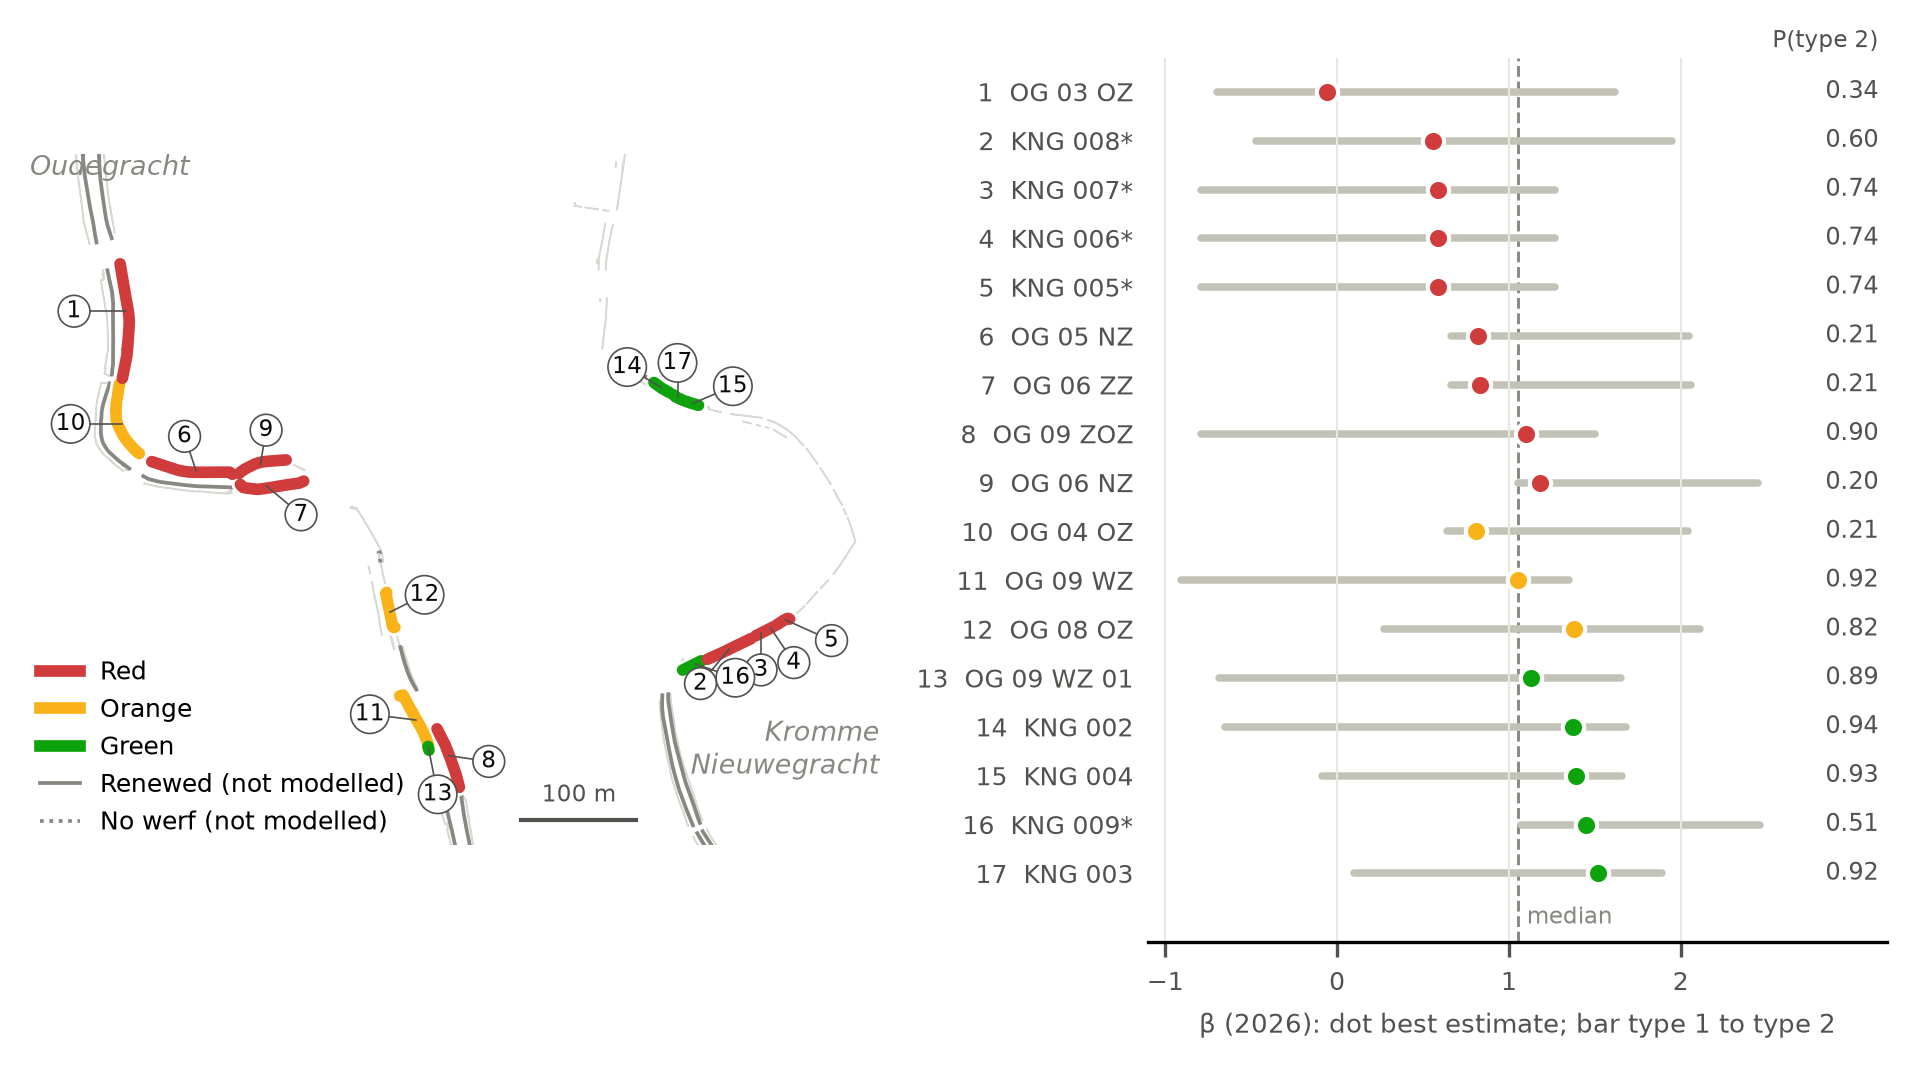
\includegraphics[width=\textwidth]{figures/results_map.png}
\caption{Risk class and $\beta$ of the 17 modelled walmuren. Right: best estimate of
$\beta$ (dot) and the range from type~1 to type~2 (bar), with the updated
probability of type~2; *: no dive note on the wall type, so the class rests on
missing data.}
\label{fig:app-results-beta}
\end{figure}

\begin{table}[htbp]
\centering
\small
\caption{Risk class of the 17 modelled walmuren. Hosp.: restaurants, cafes,
bars and outdoor seating per 100\,m; cellar: share of the wall with a cellar
front within 15\,m; road: distance to the street; scores for people, cellars
and reachability. OG = Oude Gracht, KNG = Kromme Nieuwe Gracht. *: no dive note
on the wall type; the class rests on missing data.}
\label{tab:risk-classes}
\setlength{\tabcolsep}{4pt}
\begin{tabular}{@{}r l r l r r r c l l@{}}
\toprule
 & Wall & $\beta$ & $P$ class & Hosp. & Cellar & Road [m] & Scores & Consequence & Risk \\
\midrule
1 & OG Rak 03 OZ & \textminus0.06 & high & 4.2 & 1.00 & 4.5 & 3/3/2 & high & red \\
2 & KNG 008* & 0.56 & high & 0.0 & 1.00 & 1.6 & 1/3/3 & medium & red \\
3 & KNG 007* & 0.59 & high & 0.0 & 1.00 & 1.7 & 1/3/3 & medium & red \\
4 & KNG 006* & 0.59 & high & 0.0 & 1.00 & 1.6 & 1/3/3 & medium & red \\
5 & KNG 005* & 0.59 & high & 0.0 & 1.00 & 2.8 & 1/3/3 & medium & red \\
6 & OG Rak 05 NZ & 0.82 & medium & 10.7 & 1.00 & 4.0 & 3/3/2 & high & red \\
7 & OG Rak 06 ZZ & 0.83 & medium & 4.1 & 1.00 & 3.6 & 3/3/2 & high & red \\
8 & OG Rak 09 ZOZ & 1.10 & medium & 8.5 & 1.00 & 4.3 & 3/3/2 & high & red \\
9 & OG Rak 06 NZ & 1.18 & medium & 4.8 & 1.00 & 3.1 & 3/3/2 & high & red \\
10 & OG Rak 04 OZ & 0.81 & medium & 10.2 & 1.00 & 6.7 & 3/3/1 & medium & orange \\
11 & OG Rak 09 WZ & 1.05 & medium & 6.4 & 0.39 & 13.2 & 3/2/1 & medium & orange \\
12 & OG Rak 08 OZ & 1.38 & low & 9.6 & 1.00 & 2.8 & 3/3/3 & high & orange \\
13 & OG Rak 09 WZ 01 & 1.13 & medium & 0.0 & 0.00 & 15.2 & 1/1/1 & low & green \\
14 & KNG 002 & 1.37 & low & 0.0 & 1.00 & 2.6 & 1/3/3 & medium & green \\
15 & KNG 004 & 1.39 & low & 2.0 & 1.00 & 3.2 & 2/3/2 & medium & green \\
16 & KNG 009* & 1.45 & low & 0.0 & 1.00 & 5.5 & 1/3/2 & medium & green \\
17 & KNG 003 & 1.52 & low & 2.0 & 1.00 & 4.6 & 2/3/2 & medium & green \\
\bottomrule
\end{tabular}
\end{table}

\chapter{Replacement cost regression}
\label{app:cost}

Multiple linear regression relates the replacement cost of six Dutch quay wall
projects (Table~\ref{tab:dutch-quay-walls}) to their length and to a heritage
and a disruption score, to test whether a cost that depends on the site would
be better than the cost per metre of Section~\ref{sec:tradeoff}. Lengths, works
and costs come from public sources; the disruption and heritage scores, from 1
(low) to 5 (high), were judged by the team from documented site
characteristics and are treated as equally spaced numbers.

\begin{table}[htbp]
\centering
\tiny
\caption{Characteristics and approximate replacement costs of regression quay-wall projects.}
\label{tab:dutch-quay-walls}
\setlength{\tabcolsep}{3pt}
\renewcommand{\arraystretch}{1.2}
\begin{tabular}{@{} l l r l c l c r l @{}}
\toprule
Quay wall & Replacement works & Len. & Disruption factors & Disp. & Heritage factors & Her. & Cost & References \\
\midrule
Beestenmarkt, & Full replacement of masonry & 12 & Very restricted access and & 5 & Protected historic townscape, & 4 & 0.52 & \cite{waterland2025,} \\
Monnickendam & quay; reuse of bricks. & & vehicle dimensions; pontoons. & & adjacent to historic buildings. & & & \cite{kdekker2025} \\
\addlinespace
Maaskade, & Reconstruction and raising of & 500 & Restricted parking, waterfront & 4 & Late 19th-c. quay, historic & 4 & 8.03 & \cite{maaskadeaward2018,} \\
Rotterdam & existing quay and drainage. & & works and berth loss. & & streetscape and cobblestones.  \\
\addlinespace
Haven vak M2, & Complete quay-wall and & 210 & Works in active historic harbour; & 5 & Protected townscape, demolition & 4 & 7.89 & \cite{maassluis2026,} \\
Maassluis & foundation replacement. & & public/waterway interfaces. & & permit in protected area. & & & \\
\addlinespace
Tuingracht, & Planned full replacement of & 330 & Traffic loading, parked vehicles & 4 & Nationally designated protected & 5 & 3.04 & \cite{alkmaarMIP,} \\
De Rijp & masonry wall on south bank. & & and constrained centre access. & & village centre; historic quay. & & & \cite{tuingrachtTender} \\
\addlinespace
Houtzagerssingel, & Demolition and replacement; & $\sim$370 & Utility/sewer diversions, tree & 4 & Established urban canal setting; & 3 & 6.26 & \cite{houtzagersTender,} \\
Den Haag & sheet piles, anchors, paving. & & works, pavement reinstatement. & & reinstatement of features. & & & \cite{houtzagersContractor} \\
\addlinespace
Westerkade West, & Construction of new retaining & 150 & Quayside construction and local & 3 & Historic quay dating from 1922 & 3 & 4.75 & \cite{westerkadeTender,} \\
Rotterdam & wall with steel sheet piles. & & paving/access changes. & & and waterfront character. & & & \cite{westerkadeContractor} \\
\bottomrule
\end{tabular}
\end{table}

The model explains 63.7\,\% of the variation in cost ($R^2 = 0.637$), but with
six projects and three predictors only two degrees of freedom remain for the
residuals: the adjusted $R^2$ is 0.094, and no predictor is significant at
5\,\% (length $p = 0.218$, heritage $p = 0.429$, disruption $p = 0.606$).
Forward and backward selection by AIC keep only the length ($R^2 = 0.457$), and
for a wall of 55\,m its 95\,\% prediction interval runs from \textminus\euro5.4
to \euro10.8 million. Section~\ref{sec:tradeoff} therefore keeps the cost of
about \euro35k per metre from the programme plan
\parencite{utrecht_programmaplan}.

\chapter{Municipality Summary}
\label{app:summary}

\section{Problem or decision addressed}

\noindent\fbox{%
    \parbox{\dimexpr\textwidth-2\fboxsep-2\fboxrule\relax}{%
        Utrecht has to decide where to inspect and intervene first across more
        than 60\,km of quay walls, and which measure to take (monitor, restrict
        use, strengthen or replace) until a wall is renewed, within a limited
        budget and capacity and without bringing the city to a standstill. It
        wants to stop programming on the theoretical end of life. Our method
        supports that decision by ranking walls on risk, the probability of
        failure and its consequences, with the uncertainty of the evidence made
        explicit.
    }%
}

\section{Output: type of decision support}

\noindent\fbox{%
    \parbox{\dimexpr\textwidth-2\fboxsep-2\fboxrule\relax}{%
        A traceable screening and ranking method with its code and data. For
        each wall it gives a risk class (red, orange or green) from a relative
        probability class and a consequence class, the measure that fits the
        class, and the measurement that would most change its class. For the
        test case it delivers a map and a ranked list of the 17 walmuren still on
        timber piles (Figure~\ref{fig:results-map}), the expected effect and cost
        of seven interventions (Section~\ref{sec:tradeoff}) and the risk carried
        until renewal at different paces of the programme
        (Section~\ref{sec:regression}). The level of detail is the single wall
        or rak.
    }%
}

\section{Area analysed}

\noindent\fbox{%
    \parbox{\dimexpr\textwidth-2\fboxsep-2\fboxrule\relax}{%
        The method covers the whole portfolio. It is tested on the walmuren of
        the Wervengebied along the Oudegracht, Nieuwegracht and Kromme
        Nieuwegracht: 51 walls, 4{,}062\,m in 27 raks, of which 17 walls (611\,m)
        still stand on their original timber piles with a werf. This area is used
        because only here drawings, dive records and renewal data exist to build
        and check a failure model; the wharf cellars, the street and the bridges
        are outside the system but set the consequences.
    }%
}

\section{Approach}

\noindent\fbox{%
    \parbox{\dimexpr\textwidth-2\fboxsep-2\fboxrule\relax}{%
        (1) Check the asset register: wrong, collective or rounded years,
        widths with different meanings, and renewals that are not recorded.
        (2) Renewed or recent walls are green and stay in regular inspection;
        the end of life is not used as a gate. (3) For masonry walls on timber
        piles with a werf, compute the failure probability by Monte Carlo
        simulation from the measured cross-sections, updated with the fact that
        the wall stands (proven strength); for other walls, score indicators:
        satellite movement, NEN~2767 condition, maintenance, age and data
        quality. (4) Combine the relative probability class with a consequence
        class (people on the werf, cellars, reachability) into red, orange or
        green. (5) Compare measures in a fault tree and a decision tree, and
        extrapolate the pace of renewal by regression.
    }%
}

\section{Key limitations and assumptions}

\noindent\fbox{%
    \parbox{\dimexpr\textwidth-2\fboxsep-2\fboxrule\relax}{%
        The failure model rests on two schematic cross-sections and literature
        values for the timber and the soil. It is conservative for the older wall
        type and leaves out settlement from pile rot and loss of the timber
        screen, so its results are a ranking and an order of magnitude, not a
        safety verdict under NEN~8700; that needs calibration with the wall type
        and pile condition of a sample of walls. Most human and organisational
        probabilities and the costs are team estimates, as no municipal records
        were used. The consequence score leaves out cables, pipes and trees, and
        the indicator score for walls without a model has not yet been applied
        to the rest of the portfolio.
    }%
}

\section{Why should the Municipality of Utrecht select this approach}

\noindent\fbox{%
    \parbox{\dimexpr\textwidth-2\fboxsep-2\fboxrule\relax}{%
        You want to move from a theoretical end of life to the real condition of
        your walls, but the evidence is incomplete. This approach uses what you
        already hold, the register, renewal records and open data, and shows for
        each wall how uncertain its class is and which measurement would settle
        it. In the test case it found that 11 of the 29 walmuren shown as past
        their design life were already renewed, that the unknown wall type is the
        evidence worth buying first, and that for walls due for renewal within a
        few years, keeping the edge of the werf free is the cheapest interim
        measure, while monitoring pays for walls that will wait longer. Every
        step is traceable, so choices can be explained to the council. It does
        not replace the structural assessment of a single wall, but it gives a
        defensible order in which to spend limited budget and capacity.
    }%
}


\end{document}
